\documentclass[12pt,a4paper]{article}
 
\usepackage{float}
%für feststellen der figures und tables [H] dranschreiben
\usepackage{units}
%wird so benutzt: 
%\unit[value/Zahl]{dimension/Einheit} oder 
%\unitfrac[value/Zahl]{dimension/Einheit num/Zähler}{dimension/Einheit denum/Nenner} oder
%\nicefrac[fontcommand/Schriftart]{dimension/Einheit num/Zähler}{dimension/Einheit denum/Nenner}
\usepackage[left=2cm,right=2cm,top=2cm,bottom=2cm]{geometry}
\usepackage[utf8]{inputenc}
\usepackage[T1]{fontenc}
\usepackage{lmodern}
\usepackage[ngerman]{babel}
\usepackage{amsmath}
\usepackage{graphicx}
 
\title{Versuch EP2 Die Diode}
\author{Frederik Strothmann, Henrik Jürgens}
\date{\today}
%niemals zwei überschriften direkt übereinander schreiben, also immer mindestens in einem satz was sinnvolles unter jede überschrift schreiben (bei den versuchen z.B. das versuchsziel) 
\begin{document}
%deckblatt erstellen.
\maketitle
\newpage
\tableofcontents
\newpage
\section{Einleitung}
%einleitung zu dem experiment.
%auf die einstellungen, die vor dem versuch gemacht werden, eingehen oder auf eine anleitung dazu verweisen.
%--------------------------------------------------------------------------------------------- 
%hinter der einleitung kann der allgemeine theoretische hintergrund in einer zusätzlichen section erklärt werden
In diesem Versuch geht es um die Eigenschaften von Dioden. Dazu werden im ersten Teil die Kennlinien zwei verschiedener Dioden aufgenommen. Danach werden praktische Anwendungen von Dioden untersucht, dazu gehören das Gleichrichten und Glätten von Wechselspannung, sowie das Stabilisieren einer Spannung.
\section{Eigenschaften verschiedener Dioden}
%kurz das ziel dieses versuchsteiles ansprechen, damit keine zwei überschriften direkt übereinander stehen!
%bei schwierigeren versuchen kann auch der theoretische hintergrund erläutert werden. (mit formeln, herleitungen und erklärungen)
\subsection{Verwendete Materialien}
%(immer) eine skizze oder ein foto einfügen, die geräte/materialien !nummerieren! und z.b. eine legende dazu schreiben oder besser noch das ganze in einem Fließtext gut umschreiben
%falls am anfang des versuches nicht klar ist, was alles verwendet wird, wenn möglich erst am ende ein großes foto von den verwendeten materialien machen!
\subsection{Versuchsaufbau}
%skizze zum versuchsaufbau (oder foto) einfügen,   es muss erklärt werden wie das ganze funktioniert und welche speziellen einstellungen verwendet wurden (z.b. welche knöpfe an den geräten für die messung verdreht wurden)
Im ersten Versuchsteil soll die Kennlinie einer 1N4007 Diode und einer Zenerdiode aufgenommen werden dafür wird die Schaltung aus Abbildung \ref{fig:1} verwendet. Dabei ist P$_1$ ein 10-Gang-Potentiometer, welches in 10 Schritten Widerstände von 0 bis 1k$\Omega$ annehmen kann. R$_1$ hat einen Wert von 100$\Omega$. U$_\pm$ wird mit 10V eingestellt. I$_0$ und U$_0$ sind die Strom- bzw. Spannungsmessgeräte. D bezeichnet die verwendete Diode.

\begin{figure}[H] 
  \centering
    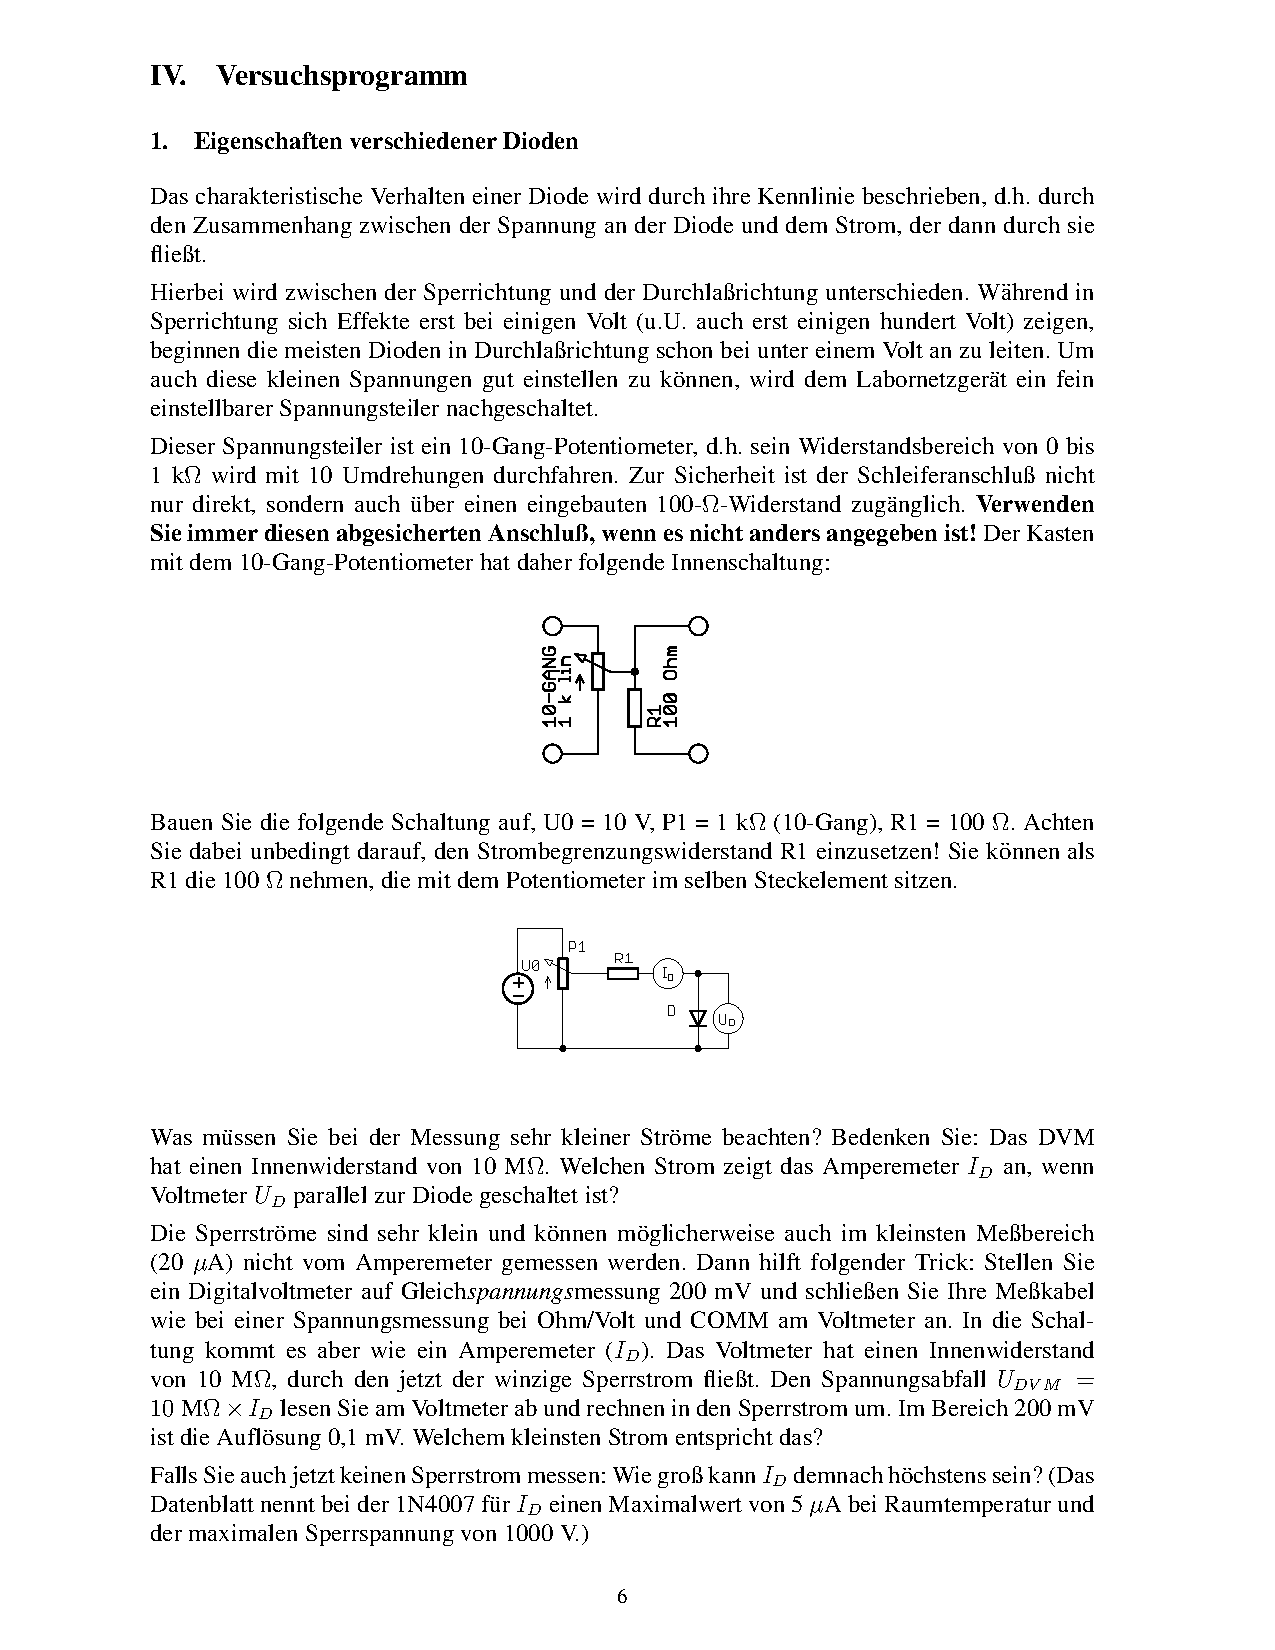
\includegraphics[trim = 10mm 100mm 10mm 155mm, clip, scale = 1]{ep2_14[Page6].pdf}
  	\caption[Schaltskizze für die Messung der Kennlinie der Dioden]{Schaltskizze für die Messung der Kennlinie der Dioden\footnotemark}
  \label{fig:1}
\end{figure}
\footnotetext{Abbildung entnommen von http://www.atlas.uni-wuppertal.de/$\sim$kind/ep2\_14.pdf Seite 6 am 28.10.2014}


\subsection{Versuchsdurchführung}
%erklären, !was! wir machen, !warum! wir das machen und mit welchem ziel
%(wichtig) präzize erklären, wie bei dem versuch vorgegangen und was gemacht wurde
\subsection{Verwendete Formeln}
%eine legende kann angefertigt werden, die selbstverständlichen buchstaben müssen nicht extra erklärt werden
%mit knappen erklärungen die !verwendeten! formeln, sowie die zugehörige fehlerrechnung einfügen.
\subsection{Messergebnisse}
%die messwerte in !übersichtlichen! tabellen angegeben
%zu viele kleine tabellen in große tabellen überführen!
%zu große tabellen mit dem [scale]-befehl scalieren oder (falls zu lang) in zwei kleinere tabellen aufteilen
%(wichtig) vor !jeder! tabelle sagen, was gemessen wurde und wie die fehler gewählt wurden und ausreichend !erklären!, !warum! wir unsere fehler grade so gewählt haben
\subsection{Auswertung}
%zuerst !alle! errechneten werte entweder in ganzen sätzen aufzählen, oder in tabellen (übersichtlicher) dargestellen, sowie auf die verwendeten formeln verweisen (die referenzierung der formel kann in der überschrift stehen)
%kurz erwähnen (vor der tabelle), warum wir das ganze ausrechnen bzw. was wir dort ausrechnen
%danach histogramme und plots erstellen, wobei wenn möglich funktionen durch die plots gelegt werden (zur not können auch splines benutzt werden, was aber angegeben werden muss)
%bei fits immer die funktion und das reduzierte chiquadrat mit angegeben, wobei auf verständlichkeit beim entziffern der zehnerpotenzen geachtet werden muss z.b. f(x)=(wert+-fehler)\cdot10^{irgendeine zahl}\cdot x + (wert+-fehler)\cdot10^{irgendeine zahl}
%bei jedem fit erklären, nach welchem zusammenhang gefittet wurde und warum!
%bei plots darauf achten, dass die achsenbeschriftung (auch die tics) die richtige größe haben und die legende im plot nicht die messwerte verdeckt
%kurz die aufgabenstellung abgehandeln
\subsection{Diskussion}
%(immer) die gemessenen werte und die bestimmten werte über die messfehler mit literaturwerten oder untereinander vergleichen
%in welchem fehlerintervall des messwertes liegt der literaturwert oder der vergleichswert?
%wie ist der relative anteil des fehlers am messwert und damit die qualität unserer messung?
%in einem satz erklären, wie gut unser fehler und damit unsere messung ist
%kurz erläutern, wie systematische fehler unsere messung beeinflusst haben könnten
%(wichtig) zum schluss ansprechen, in wie weit die ergebnisse mit der theoretischen vorhersage übereinstimmen
%--------------------------------------------------------------------------------------------
%falls tabellen mit den messwerten zu lang werden, kann die section mit den messwerten auch hinter der diskussion angefügt bzw. eine section mit dem anhang eingefügt werden.
\section{Gleichrichterschaltungen}
%kurz das ziel dieses versuchsteiles ansprechen, damit keine zwei überschriften direkt übereinander stehen!
%bei schwierigeren versuchen kann auch der theoretische hintergrund erläutert werden. (mit formeln, herleitungen und erklärungen)
\subsection{Verwendete Formeln}
%eine legende kann angefertigt werden, die selbstverständlichen buchstaben müssen nicht extra erklärt werden
%mit knappen erklärungen die !verwendeten! formeln, sowie die zugehörige fehlerrechnung einfügen.
\subsection{Verwendete Materialien}
%(immer) eine skizze oder ein foto einfügen, die geräte/materialien !nummerieren! und z.b. eine legende dazu schreiben oder besser noch das ganze in einem Fließtext gut umschreiben
%falls am anfang des versuches nicht klar ist, was alles verwendet wird, wenn möglich erst am ende ein großes foto von den verwendeten materialien machen!
\subsection{Einweggleichrichtung (Sinusgenerator)}
In diesem Versuchsteil soll das Gleichrichten einer Sinusspannung mittels einer Diode untersucht werden.
\subsubsection{Versuchsaufbau}
%skizze zum versuchsaufbau (oder foto) einfügen,   es muss erklärt werden wie das ganze funktioniert und welche speziellen einstellungen verwendet wurden (z.b. welche knöpfe an den geräten für die messung verdreht wurden)
In diesem Aufbau wird die 1N4007 Diode verwendet. R$_\text{L}$ hat einen Widerstand von 10k$\Omega$. Es werden Frequenzen von 50Hz bis 10kHz durchfahren. Der genaue Aufbau ist Abbildung ?? zu entnahmen.

\begin{figure}[H] 
  \centering
    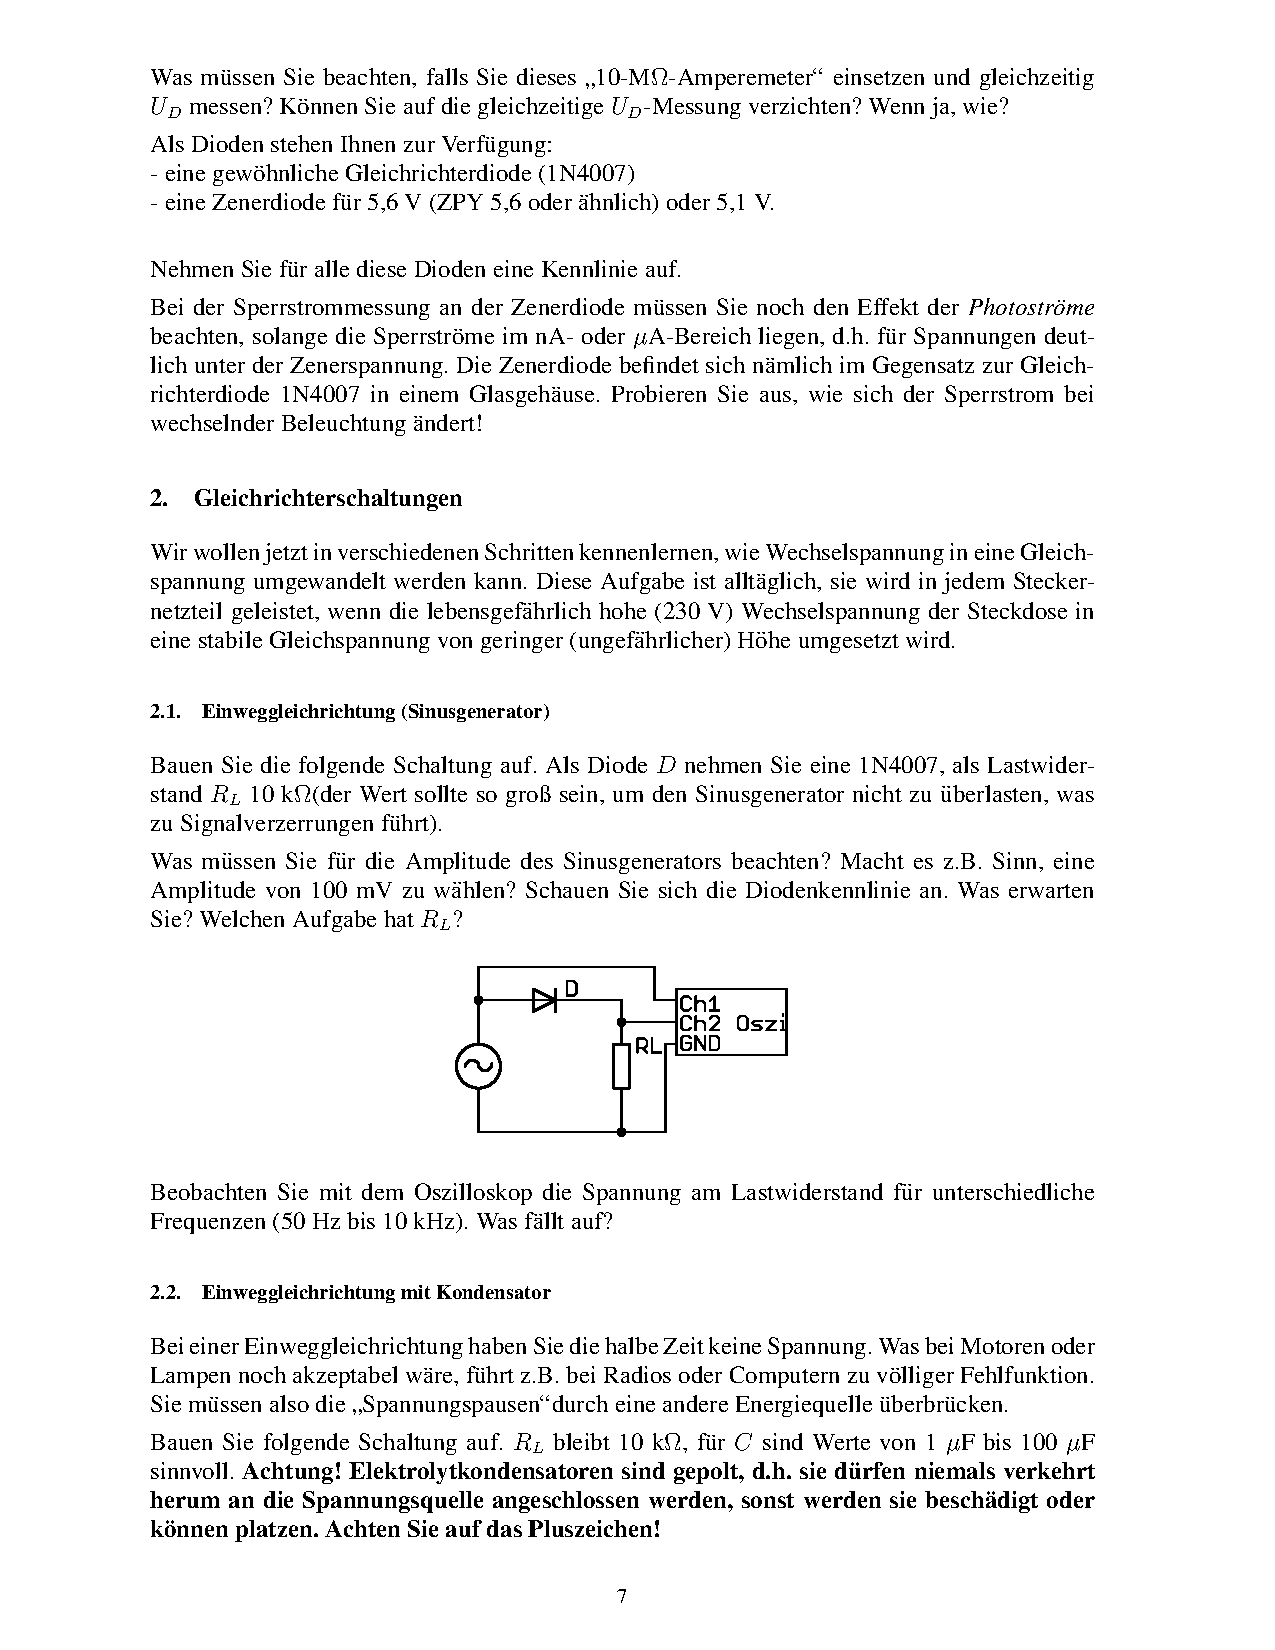
\includegraphics[trim = 10mm 80mm 10mm 160mm, clip, scale = 1]{ep2_14[Page7].pdf}
  	\caption[Schaltskizze für die Messung der Spannung am Lastwiderstand nach vorgeschalteter Diode]{Schaltskizze für die Messung der Spannung am Lastwiderstand nach vorgeschalteter Diode\footnotemark}
  \label{fig:2_1}
\end{figure}
\footnotetext{Abbildung entnommen von http://www.atlas.uni-wuppertal.de/$\sim$kind/ep2\_14.pdf Seite 7 am 28.10.2014}
\subsubsection{Versuchsdurchführung}
%erklären, !was! wir machen, !warum! wir das machen und mit welchem ziel
%(wichtig) präzize erklären, wie bei dem versuch vorgegangen und was gemacht wurde

\subsubsection{Messergebnisse}
%die messwerte in !übersichtlichen! tabellen angegeben
%zu viele kleine tabellen in große tabellen überführen!
%zu große tabellen mit dem [scale]-befehl scalieren oder (falls zu lang) in zwei kleinere tabellen aufteilen
%(wichtig) vor !jeder! tabelle sagen, was gemessen wurde und wie die fehler gewählt wurden und ausreichend !erklären!, !warum! wir unsere fehler grade so gewählt haben
\subsubsection{Auswertung}
%zuerst !alle! errechneten werte entweder in ganzen sätzen aufzählen, oder in tabellen (übersichtlicher) dargestellen, sowie auf die verwendeten formeln verweisen (die referenzierung der formel kann in der überschrift stehen)
%kurz erwähnen (vor der tabelle), warum wir das ganze ausrechnen bzw. was wir dort ausrechnen
%danach histogramme und plots erstellen, wobei wenn möglich funktionen durch die plots gelegt werden (zur not können auch splines benutzt werden, was aber angegeben werden muss)
%bei fits immer die funktion und das reduzierte chiquadrat mit angegeben, wobei auf verständlichkeit beim entziffern der zehnerpotenzen geachtet werden muss z.b. f(x)=(wert+-fehler)\cdot10^{irgendeine zahl}\cdot x + (wert+-fehler)\cdot10^{irgendeine zahl}
%bei jedem fit erklären, nach welchem zusammenhang gefittet wurde und warum!
%bei plots darauf achten, dass die achsenbeschriftung (auch die tics) die richtige größe haben und die legende im plot nicht die messwerte verdeckt
%kurz die aufgabenstellung abgehandeln
\subsection{Einweggleichrichtung mit Kondensator}
\subsubsection{Versuchsaufbau}
%skizze zum versuchsaufbau (oder foto) einfügen,   es muss erklärt werden wie das ganze funktioniert und welche speziellen einstellungen verwendet wurden (z.b. welche knöpfe an den geräten für die messung verdreht wurden)
Es wird der selbe Versuchsaufbau wie in Abbildung \ref{fig:2_1} Verwendet, jedoch wird noch ein hinter der Diode liegender Kondensator parallel zu R$_\text{L}$ geschaltet. Für den Kondensator sind Werte von 1$\mu$F bis 100$\mu$F verwendbar.
\begin{figure}[H] 
  \centering
    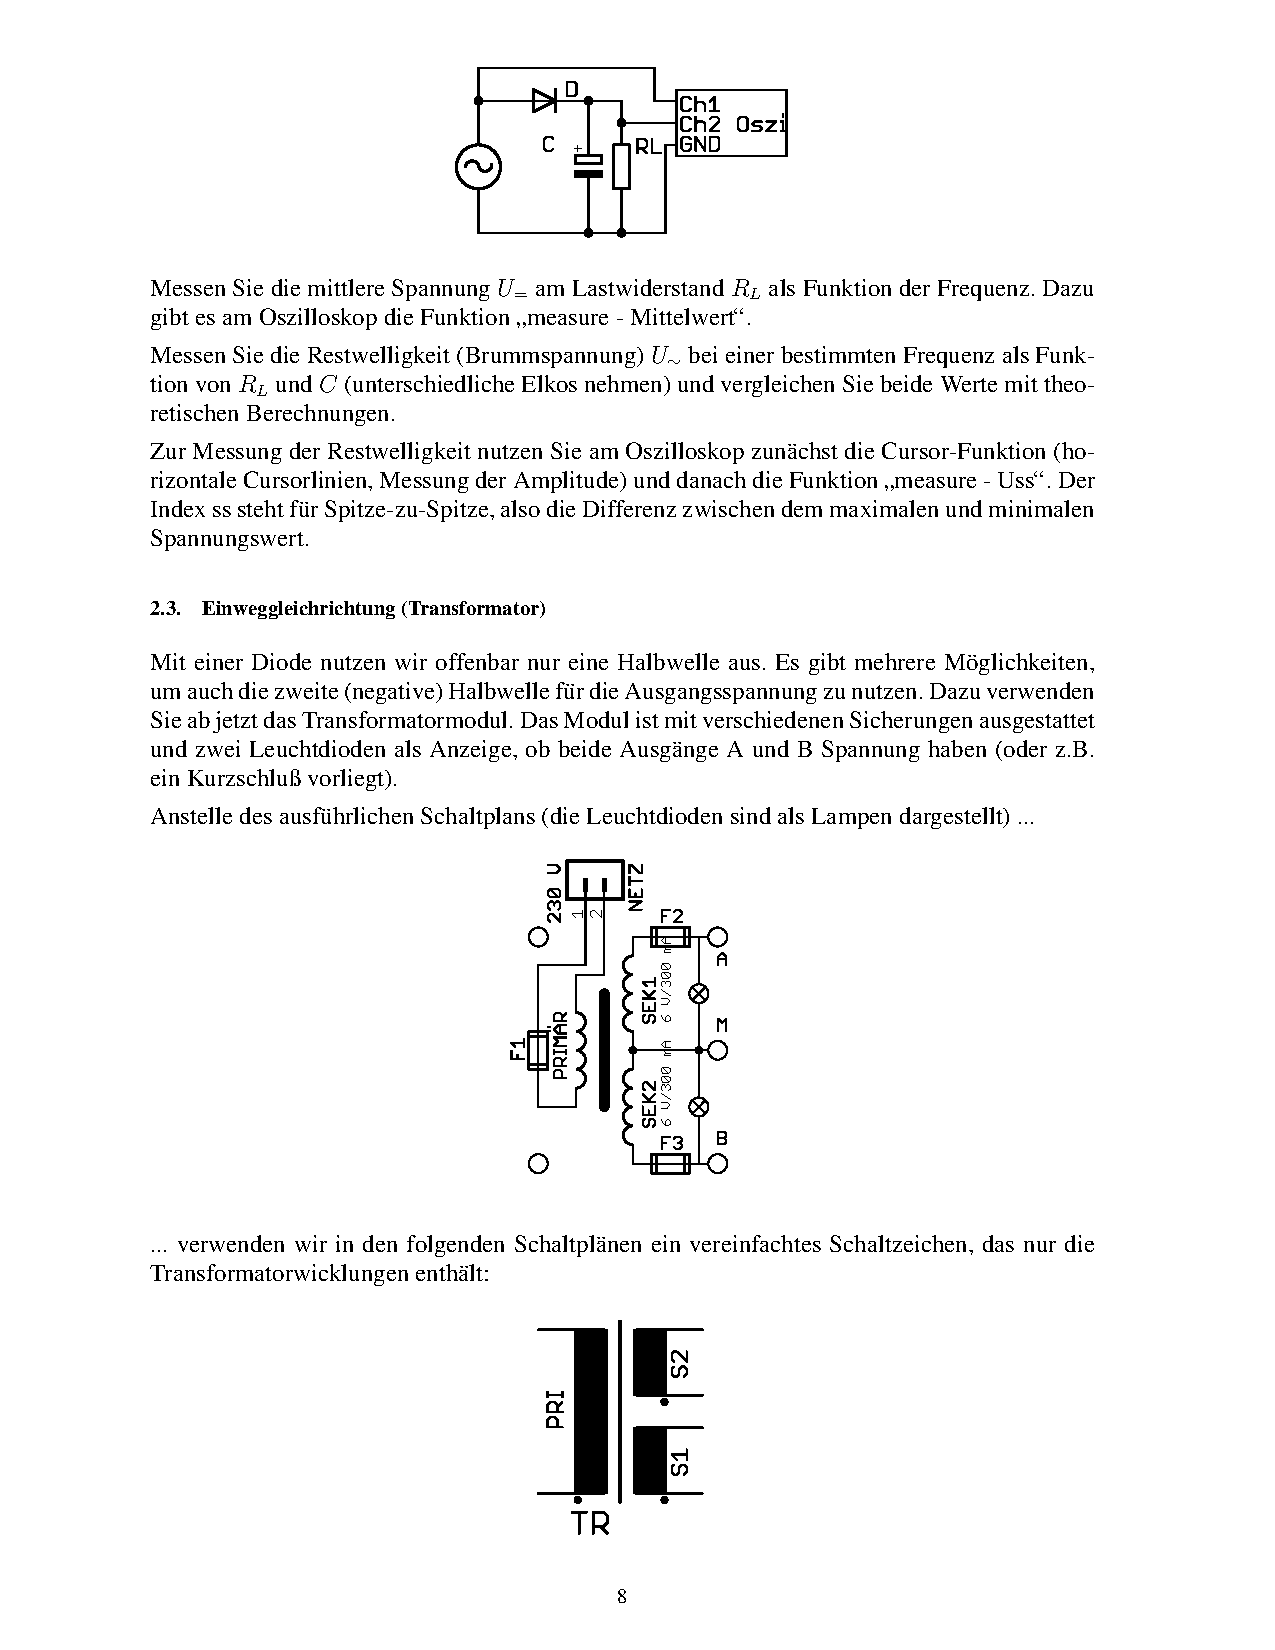
\includegraphics[trim = 10mm 235mm 10mm 10mm, clip, scale = 1]{ep2_14[Page8].pdf}
  	\caption[Schaltskizze für die Messung der Eigenschaften einer Einweggleichrichtungsschaltung mit Kondensator]{Schaltskizze für die Messung der Eigenschaften einer Einweggleichrichtungsschaltung mit Kondensator\footnotemark}
  \label{fig:2_2}
\end{figure}
\footnotetext{Abbildung entnommen von http://www.atlas.uni-wuppertal.de/$\sim$kind/ep2\_14.pdf Seite 8 am 28.10.2014}

\subsubsection{Versuchsdurchführung}
%erklären, !was! wir machen, !warum! wir das machen und mit welchem ziel
%(wichtig) präzize erklären, wie bei dem versuch vorgegangen und was gemacht wurde

\subsubsection{Messergebnisse}
%die messwerte in !übersichtlichen! tabellen angegeben
%zu viele kleine tabellen in große tabellen überführen!
%zu große tabellen mit dem [scale]-befehl scalieren oder (falls zu lang) in zwei kleinere tabellen aufteilen
%(wichtig) vor !jeder! tabelle sagen, was gemessen wurde und wie die fehler gewählt wurden und ausreichend !erklären!, !warum! wir unsere fehler grade so gewählt haben
\subsubsection{Auswertung}
%zuerst !alle! errechneten werte entweder in ganzen sätzen aufzählen, oder in tabellen (übersichtlicher) dargestellen, sowie auf die verwendeten formeln verweisen (die referenzierung der formel kann in der überschrift stehen)
%kurz erwähnen (vor der tabelle), warum wir das ganze ausrechnen bzw. was wir dort ausrechnen
%danach histogramme und plots erstellen, wobei wenn möglich funktionen durch die plots gelegt werden (zur not können auch splines benutzt werden, was aber angegeben werden muss)
%bei fits immer die funktion und das reduzierte chiquadrat mit angegeben, wobei auf verständlichkeit beim entziffern der zehnerpotenzen geachtet werden muss z.b. f(x)=(wert+-fehler)\cdot10^{irgendeine zahl}\cdot x + (wert+-fehler)\cdot10^{irgendeine zahl}
%bei jedem fit erklären, nach welchem zusammenhang gefittet wurde und warum!
%bei plots darauf achten, dass die achsenbeschriftung (auch die tics) die richtige größe haben und die legende im plot nicht die messwerte verdeckt
%kurz die aufgabenstellung abgehandeln

\subsection{Einweggleichrichtung (Transformator)}
\subsubsection{Versuchsaufbau}
%skizze zum versuchsaufbau (oder foto) einfügen,   es muss erklärt werden wie das ganze funktioniert und welche speziellen einstellungen verwendet wurden (z.b. welche knöpfe an den geräten für die messung verdreht wurden)

\begin{figure}[H] 
  \centering
    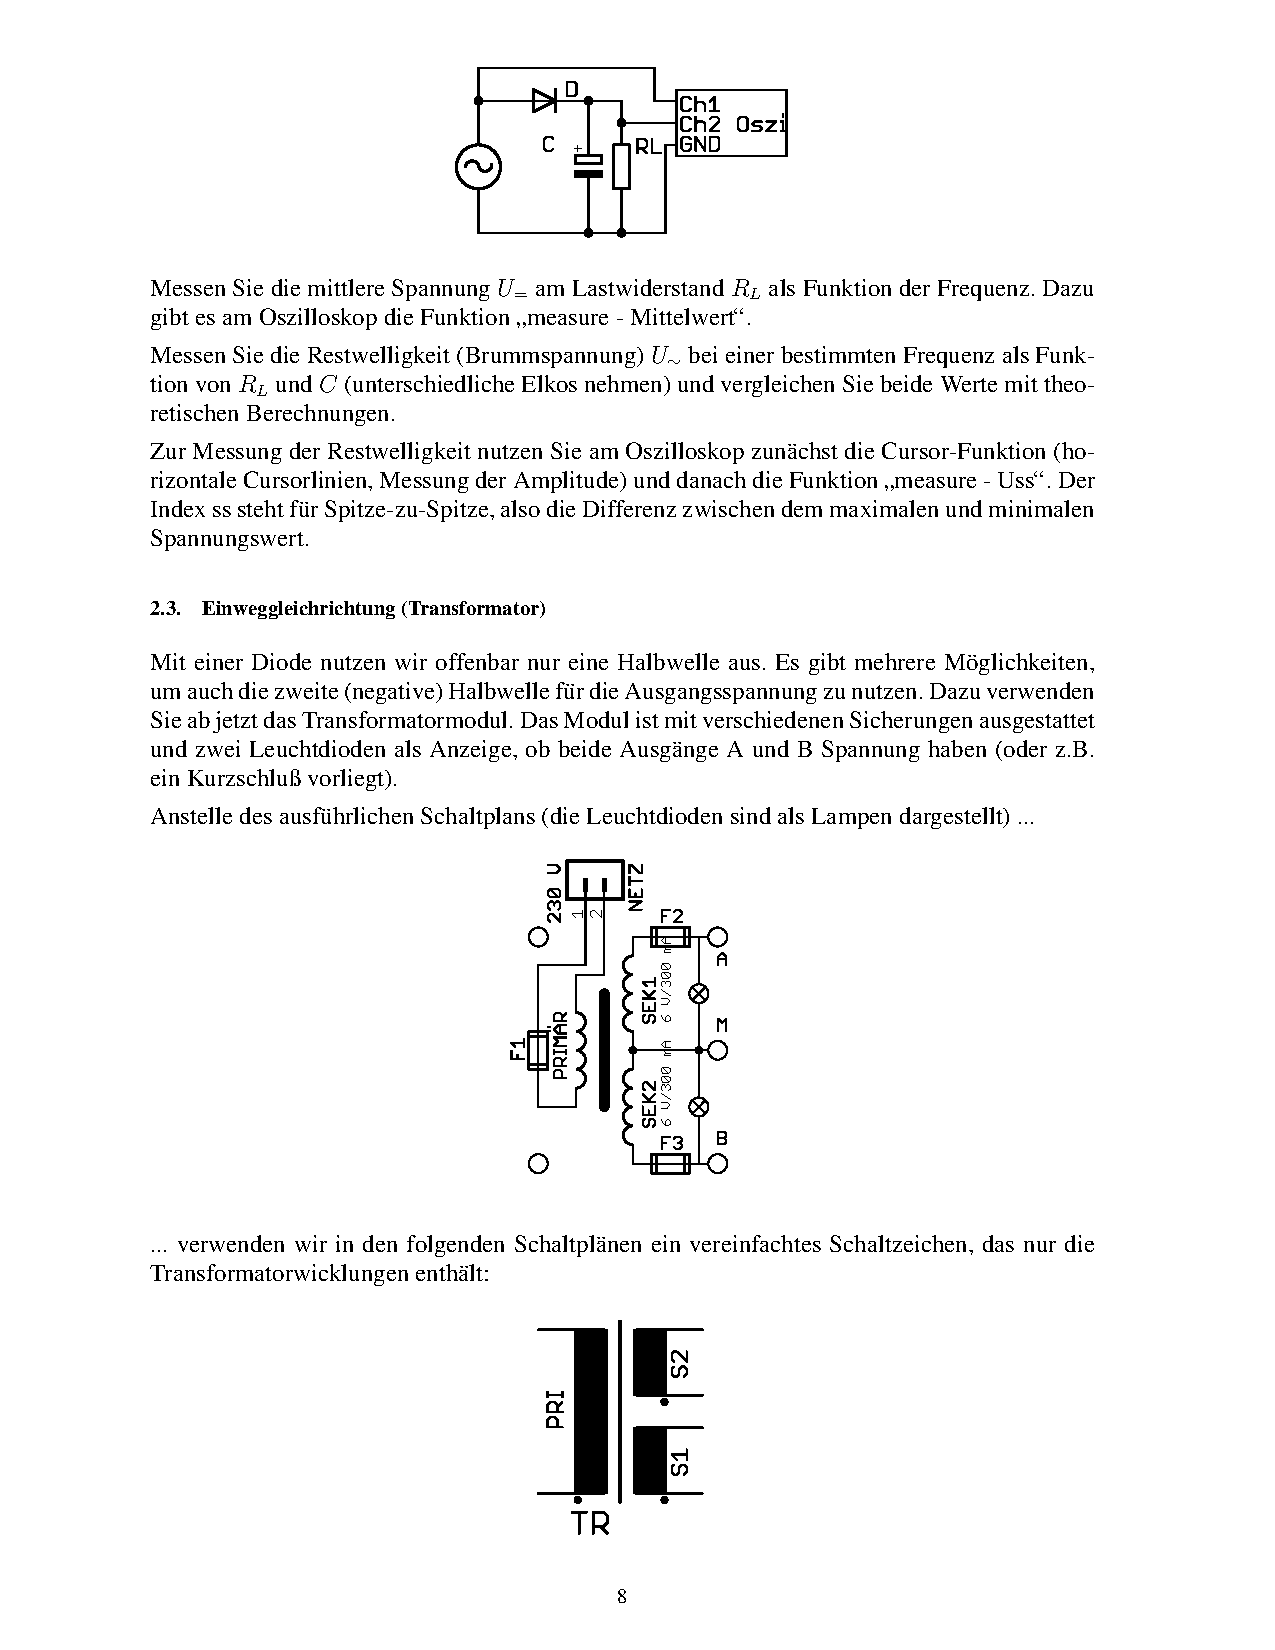
\includegraphics[trim = 10mm 75mm 10mm 145mm, clip, scale = 1]{ep2_14[Page8].pdf}
  	\caption[Schaltskizze für die Messung der Eigenschaften einer Einweggleichrichtungsschaltung mit Transformator]{Schaltskizze für die Messung der Eigenschaften einer Einweggleichrichtungsschaltung mit Transformator\footnotemark}
  \label{fig:2_3}
\end{figure}
\footnotetext{Abbildung entnommen von http://www.atlas.uni-wuppertal.de/$\sim$kind/ep2\_14.pdf Seite 8 am 28.10.2014}


\begin{figure}[H] 
  \centering
    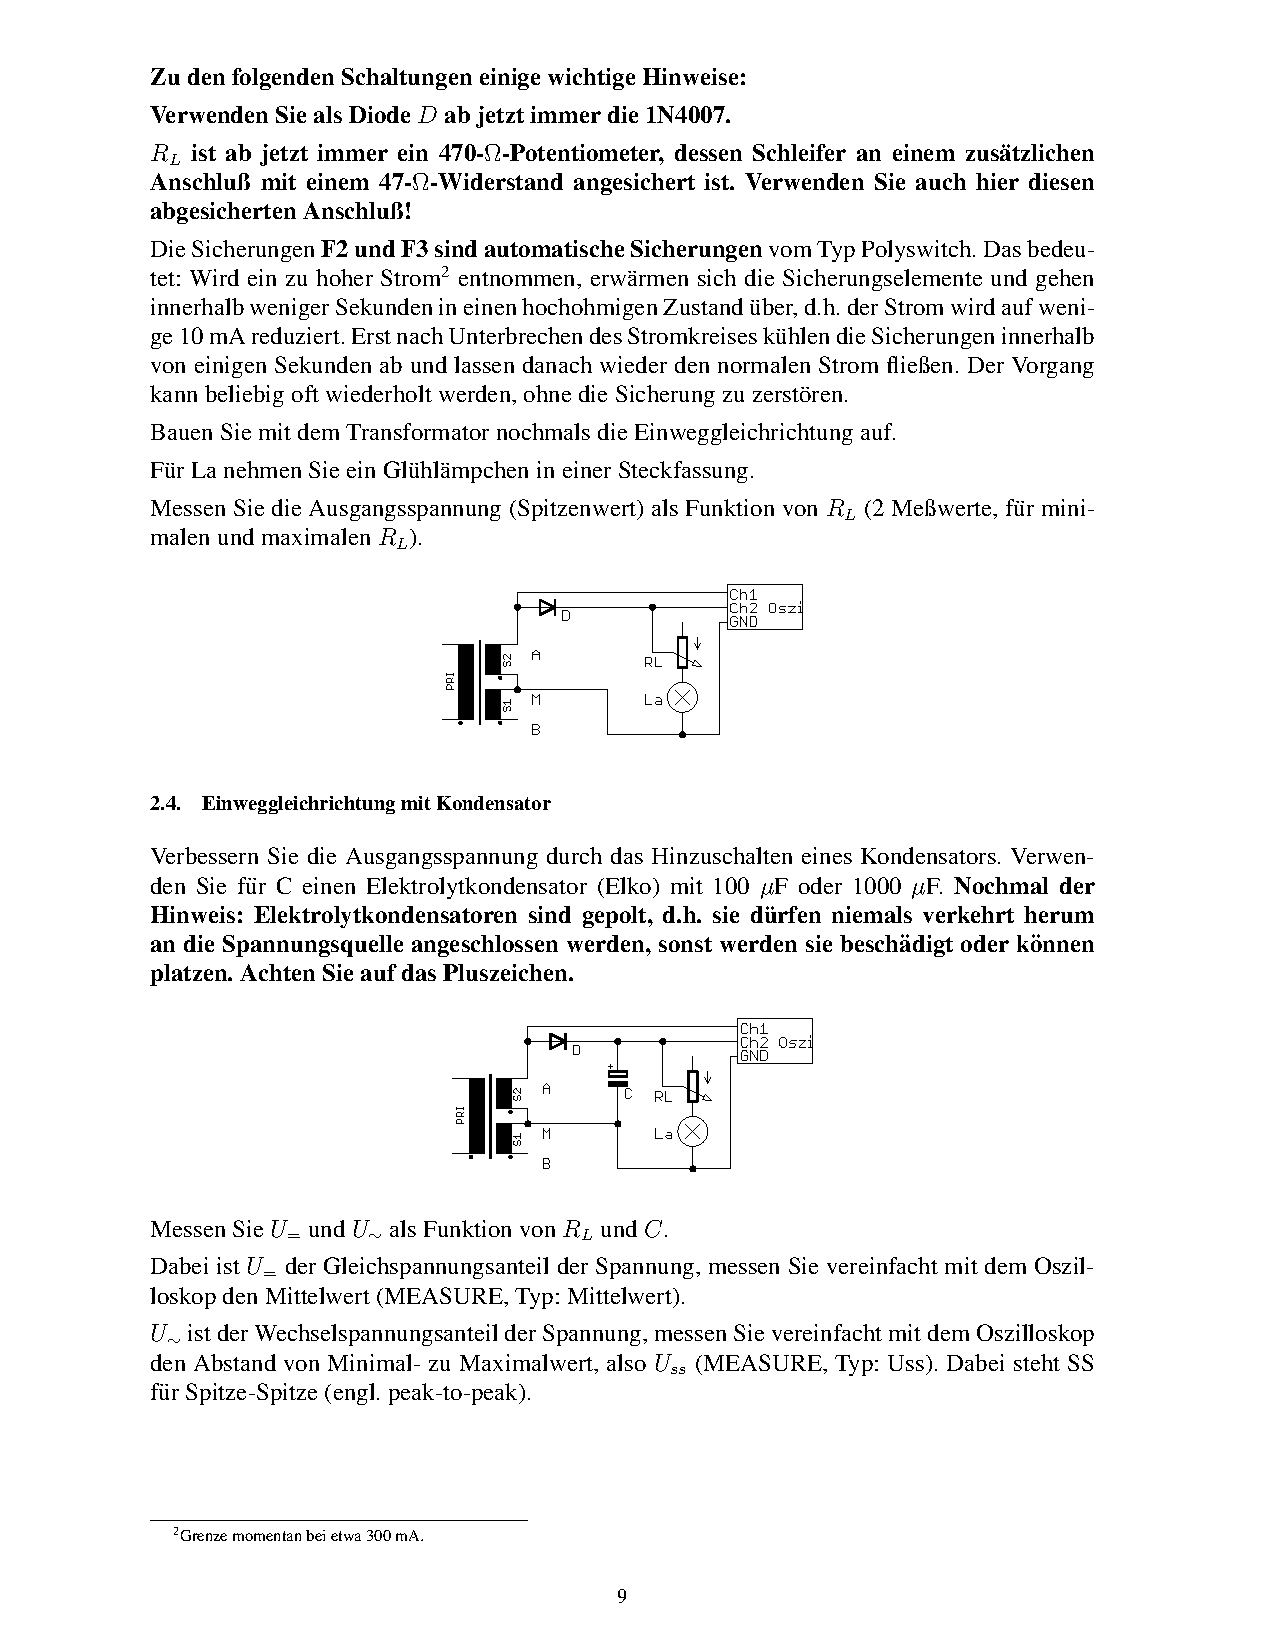
\includegraphics[trim = 10mm 150mm 10mm 95mm, clip, scale = 1]{ep2_14[Page9].pdf}
  	\caption[Schaltskizze für die Messung der Eigenschaften einer Einweggleichrichtungsschaltung mit Transformator]{Schaltskizze für die Messung der Eigenschaften einer Einweggleichrichtungsschaltung mit Transformator\footnotemark}
  \label{fig:2_4}
\end{figure}
\footnotetext{Abbildung entnommen von http://www.atlas.uni-wuppertal.de/$\sim$kind/ep2\_14.pdf Seite 9 am 28.10.2014}

\subsubsection{Versuchsdurchführung}
%erklären, !was! wir machen, !warum! wir das machen und mit welchem ziel
%(wichtig) präzize erklären, wie bei dem versuch vorgegangen und was gemacht wurde
\subsubsection{Messergebnisse}
%die messwerte in !übersichtlichen! tabellen angegeben
%zu viele kleine tabellen in große tabellen überführen!
%zu große tabellen mit dem [scale]-befehl scalieren oder (falls zu lang) in zwei kleinere tabellen aufteilen
%(wichtig) vor !jeder! tabelle sagen, was gemessen wurde und wie die fehler gewählt wurden und ausreichend !erklären!, !warum! wir unsere fehler grade so gewählt haben
\subsubsection{Auswertung}
%zuerst !alle! errechneten werte entweder in ganzen sätzen aufzählen, oder in tabellen (übersichtlicher) dargestellen, sowie auf die verwendeten formeln verweisen (die referenzierung der formel kann in der überschrift stehen)
%kurz erwähnen (vor der tabelle), warum wir das ganze ausrechnen bzw. was wir dort ausrechnen
%danach histogramme und plots erstellen, wobei wenn möglich funktionen durch die plots gelegt werden (zur not können auch splines benutzt werden, was aber angegeben werden muss)
%bei fits immer die funktion und das reduzierte chiquadrat mit angegeben, wobei auf verständlichkeit beim entziffern der zehnerpotenzen geachtet werden muss z.b. f(x)=(wert+-fehler)\cdot10^{irgendeine zahl}\cdot x + (wert+-fehler)\cdot10^{irgendeine zahl}
%bei jedem fit erklären, nach welchem zusammenhang gefittet wurde und warum!
%bei plots darauf achten, dass die achsenbeschriftung (auch die tics) die richtige größe haben und die legende im plot nicht die messwerte verdeckt
%kurz die aufgabenstellung abgehandeln
\subsection{Einweggleichrichtung mit Kondensator}
\subsubsection{Versuchsaufbau}
%skizze zum versuchsaufbau (oder foto) einfügen,   es muss erklärt werden wie das ganze funktioniert und welche speziellen einstellungen verwendet wurden (z.b. welche knöpfe an den geräten für die messung verdreht wurden)

\begin{figure}[H] 
  \centering
    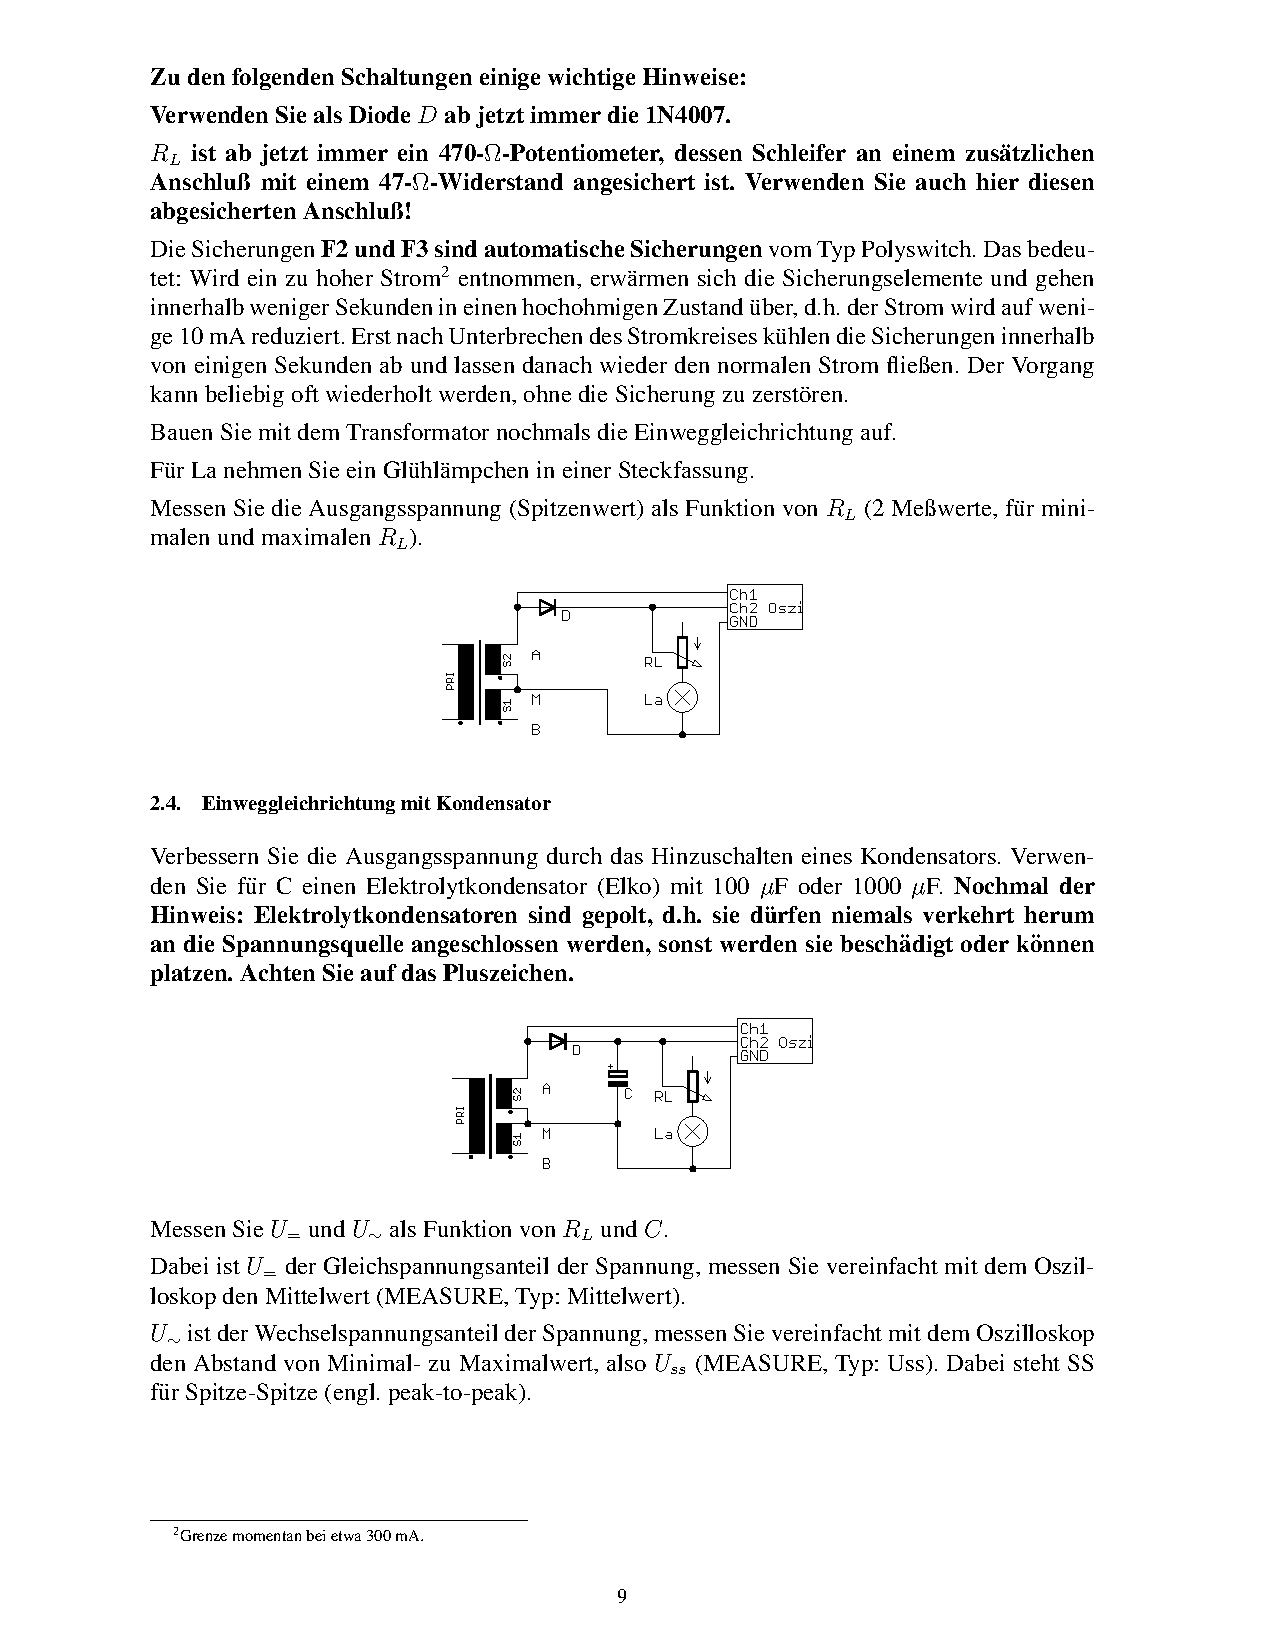
\includegraphics[trim = 10mm 150mm 10mm 95mm, clip, scale = 1]{ep2_14[Page9].pdf}
  	\caption[Schaltskizze für die Messung der Eigenschaften einer Einweggleichrichtungsschaltung mit Transformator]{Schaltskizze für die Messung der Eigenschaften einer Einweggleichrichtungsschaltung mit Transformator\footnotemark}
  \label{fig:2_5}
\end{figure}
\footnotetext{Abbildung entnommen von http://www.atlas.uni-wuppertal.de/$\sim$kind/ep2\_14.pdf Seite 9 am 28.10.2014}

\subsubsection{Versuchsdurchführung}
%erklären, !was! wir machen, !warum! wir das machen und mit welchem ziel
%(wichtig) präzize erklären, wie bei dem versuch vorgegangen und was gemacht wurde

\subsubsection{Messergebnisse}
%die messwerte in !übersichtlichen! tabellen angegeben
%zu viele kleine tabellen in große tabellen überführen!
%zu große tabellen mit dem [scale]-befehl scalieren oder (falls zu lang) in zwei kleinere tabellen aufteilen
%(wichtig) vor !jeder! tabelle sagen, was gemessen wurde und wie die fehler gewählt wurden und ausreichend !erklären!, !warum! wir unsere fehler grade so gewählt haben
\subsubsection{Auswertung}
%zuerst !alle! errechneten werte entweder in ganzen sätzen aufzählen, oder in tabellen (übersichtlicher) dargestellen, sowie auf die verwendeten formeln verweisen (die referenzierung der formel kann in der überschrift stehen)
%kurz erwähnen (vor der tabelle), warum wir das ganze ausrechnen bzw. was wir dort ausrechnen
%danach histogramme und plots erstellen, wobei wenn möglich funktionen durch die plots gelegt werden (zur not können auch splines benutzt werden, was aber angegeben werden muss)
%bei fits immer die funktion und das reduzierte chiquadrat mit angegeben, wobei auf verständlichkeit beim entziffern der zehnerpotenzen geachtet werden muss z.b. f(x)=(wert+-fehler)\cdot10^{irgendeine zahl}\cdot x + (wert+-fehler)\cdot10^{irgendeine zahl}
%bei jedem fit erklären, nach welchem zusammenhang gefittet wurde und warum!
%bei plots darauf achten, dass die achsenbeschriftung (auch die tics) die richtige größe haben und die legende im plot nicht die messwerte verdeckt
%kurz die aufgabenstellung abgehandeln
\subsection{Doppelweggleichrichtung mit Kondensator}
\subsubsection{Versuchsaufbau}
%skizze zum versuchsaufbau (oder foto) einfügen,   es muss erklärt werden wie das ganze funktioniert und welche speziellen einstellungen verwendet wurden (z.b. welche knöpfe an den geräten für die messung verdreht wurden)

\begin{figure}[H] 
  \centering
    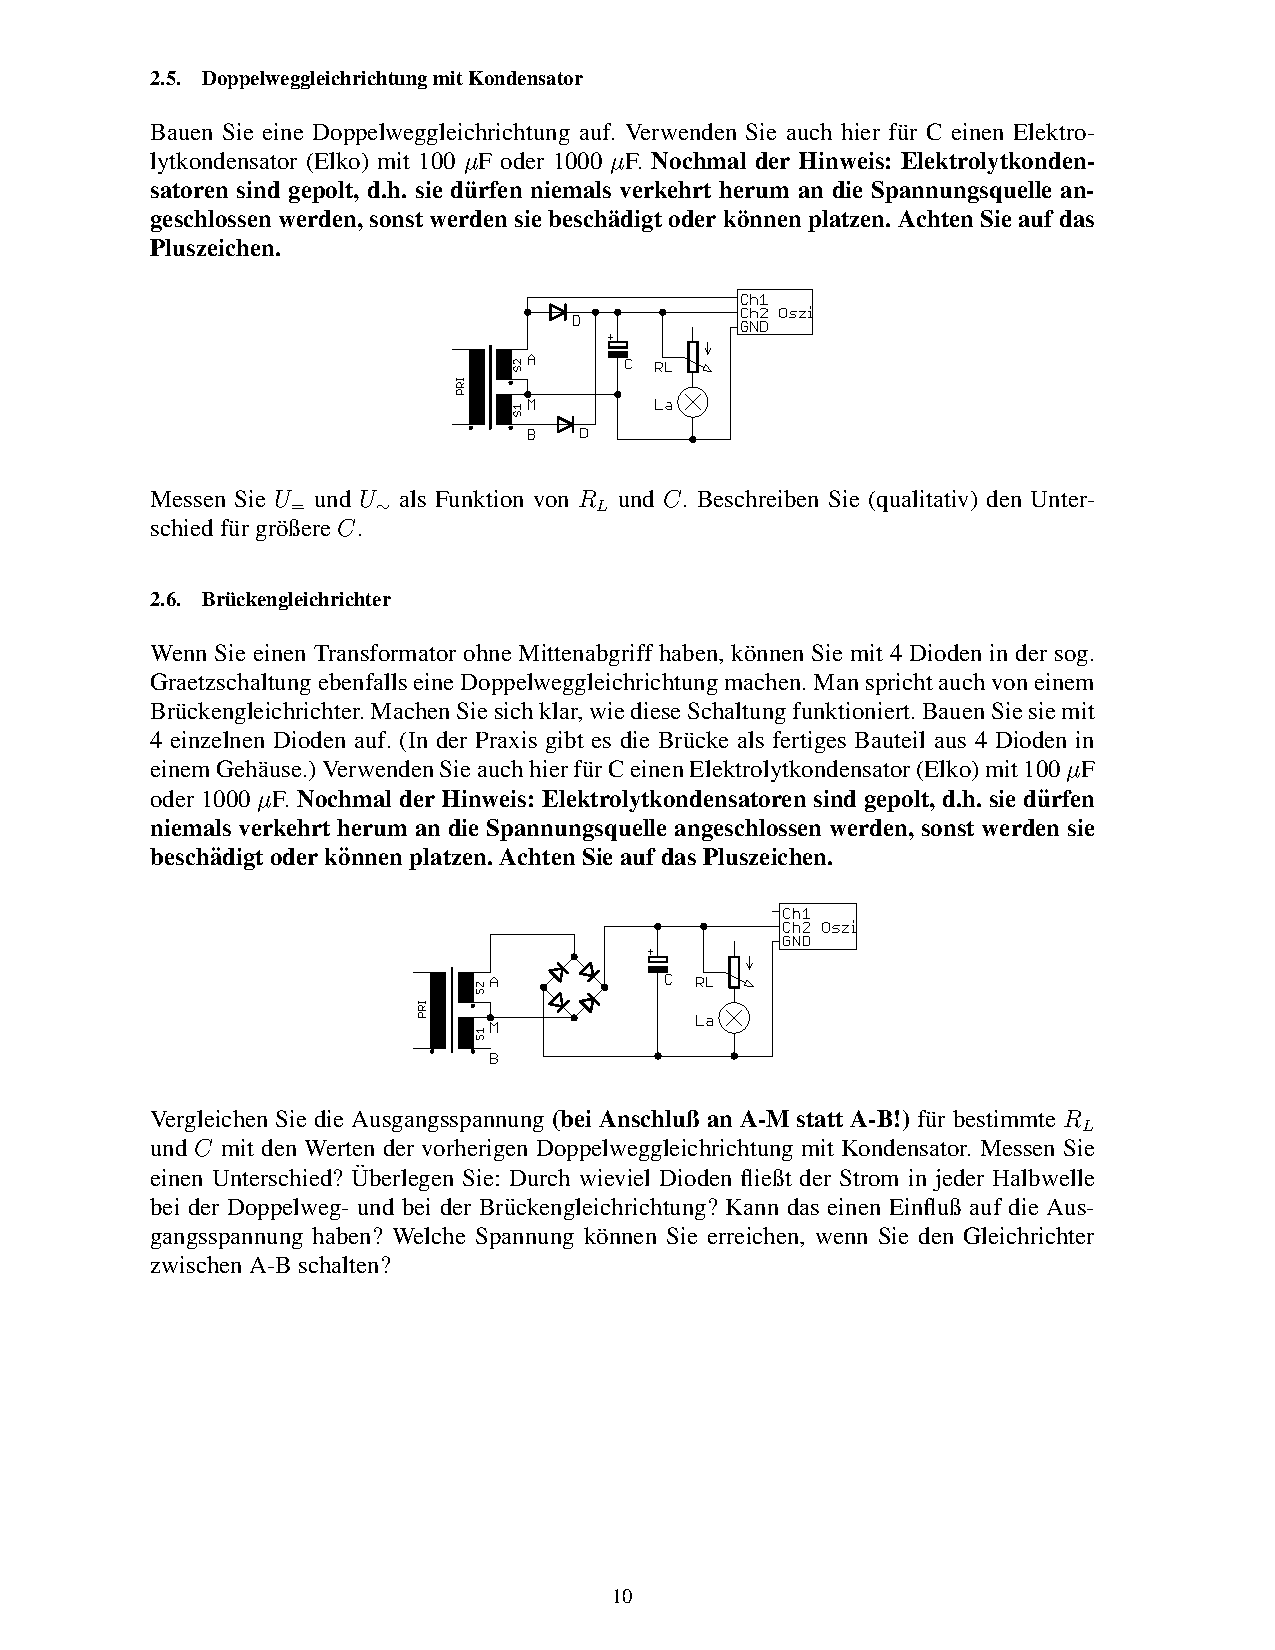
\includegraphics[trim = 10mm 200mm 10mm 45mm, clip, scale = 1]{ep2_14[Page10].pdf}
  	\caption[Schaltskizze für die Messung der Eigenschaften einer Einweggleichrichtungsschaltung mit Transformator]{Schaltskizze für die Messung der Eigenschaften einer Einweggleichrichtungsschaltung mit Transformator\footnotemark}
  \label{fig:2_6}
\end{figure}
\footnotetext{Abbildung entnommen von http://www.atlas.uni-wuppertal.de/$\sim$kind/ep2\_14.pdf Seite 10 am 28.10.2014}

\subsubsection{Versuchsdurchführung}
%erklären, !was! wir machen, !warum! wir das machen und mit welchem ziel
%(wichtig) präzize erklären, wie bei dem versuch vorgegangen und was gemacht wurde
\subsubsection{Messergebnisse}
%die messwerte in !übersichtlichen! tabellen angegeben
%zu viele kleine tabellen in große tabellen überführen!
%zu große tabellen mit dem [scale]-befehl scalieren oder (falls zu lang) in zwei kleinere tabellen aufteilen
%(wichtig) vor !jeder! tabelle sagen, was gemessen wurde und wie die fehler gewählt wurden und ausreichend !erklären!, !warum! wir unsere fehler grade so gewählt haben
\subsubsection{Auswertung}
%zuerst !alle! errechneten werte entweder in ganzen sätzen aufzählen, oder in tabellen (übersichtlicher) dargestellen, sowie auf die verwendeten formeln verweisen (die referenzierung der formel kann in der überschrift stehen)
%kurz erwähnen (vor der tabelle), warum wir das ganze ausrechnen bzw. was wir dort ausrechnen
%danach histogramme und plots erstellen, wobei wenn möglich funktionen durch die plots gelegt werden (zur not können auch splines benutzt werden, was aber angegeben werden muss)
%bei fits immer die funktion und das reduzierte chiquadrat mit angegeben, wobei auf verständlichkeit beim entziffern der zehnerpotenzen geachtet werden muss z.b. f(x)=(wert+-fehler)\cdot10^{irgendeine zahl}\cdot x + (wert+-fehler)\cdot10^{irgendeine zahl}
%bei jedem fit erklären, nach welchem zusammenhang gefittet wurde und warum!
%bei plots darauf achten, dass die achsenbeschriftung (auch die tics) die richtige größe haben und die legende im plot nicht die messwerte verdeckt
%kurz die aufgabenstellung abgehandeln
\subsection{Brückengleichrichter}
\subsubsection{Verwendete Materialien}
\subsubsection{Versuchsaufbau}
%skizze zum versuchsaufbau (oder foto) einfügen,   es muss erklärt werden wie das ganze funktioniert und welche speziellen einstellungen verwendet wurden (z.b. welche knöpfe an den geräten für die messung verdreht wurden)

\begin{figure}[H] 
  \centering
    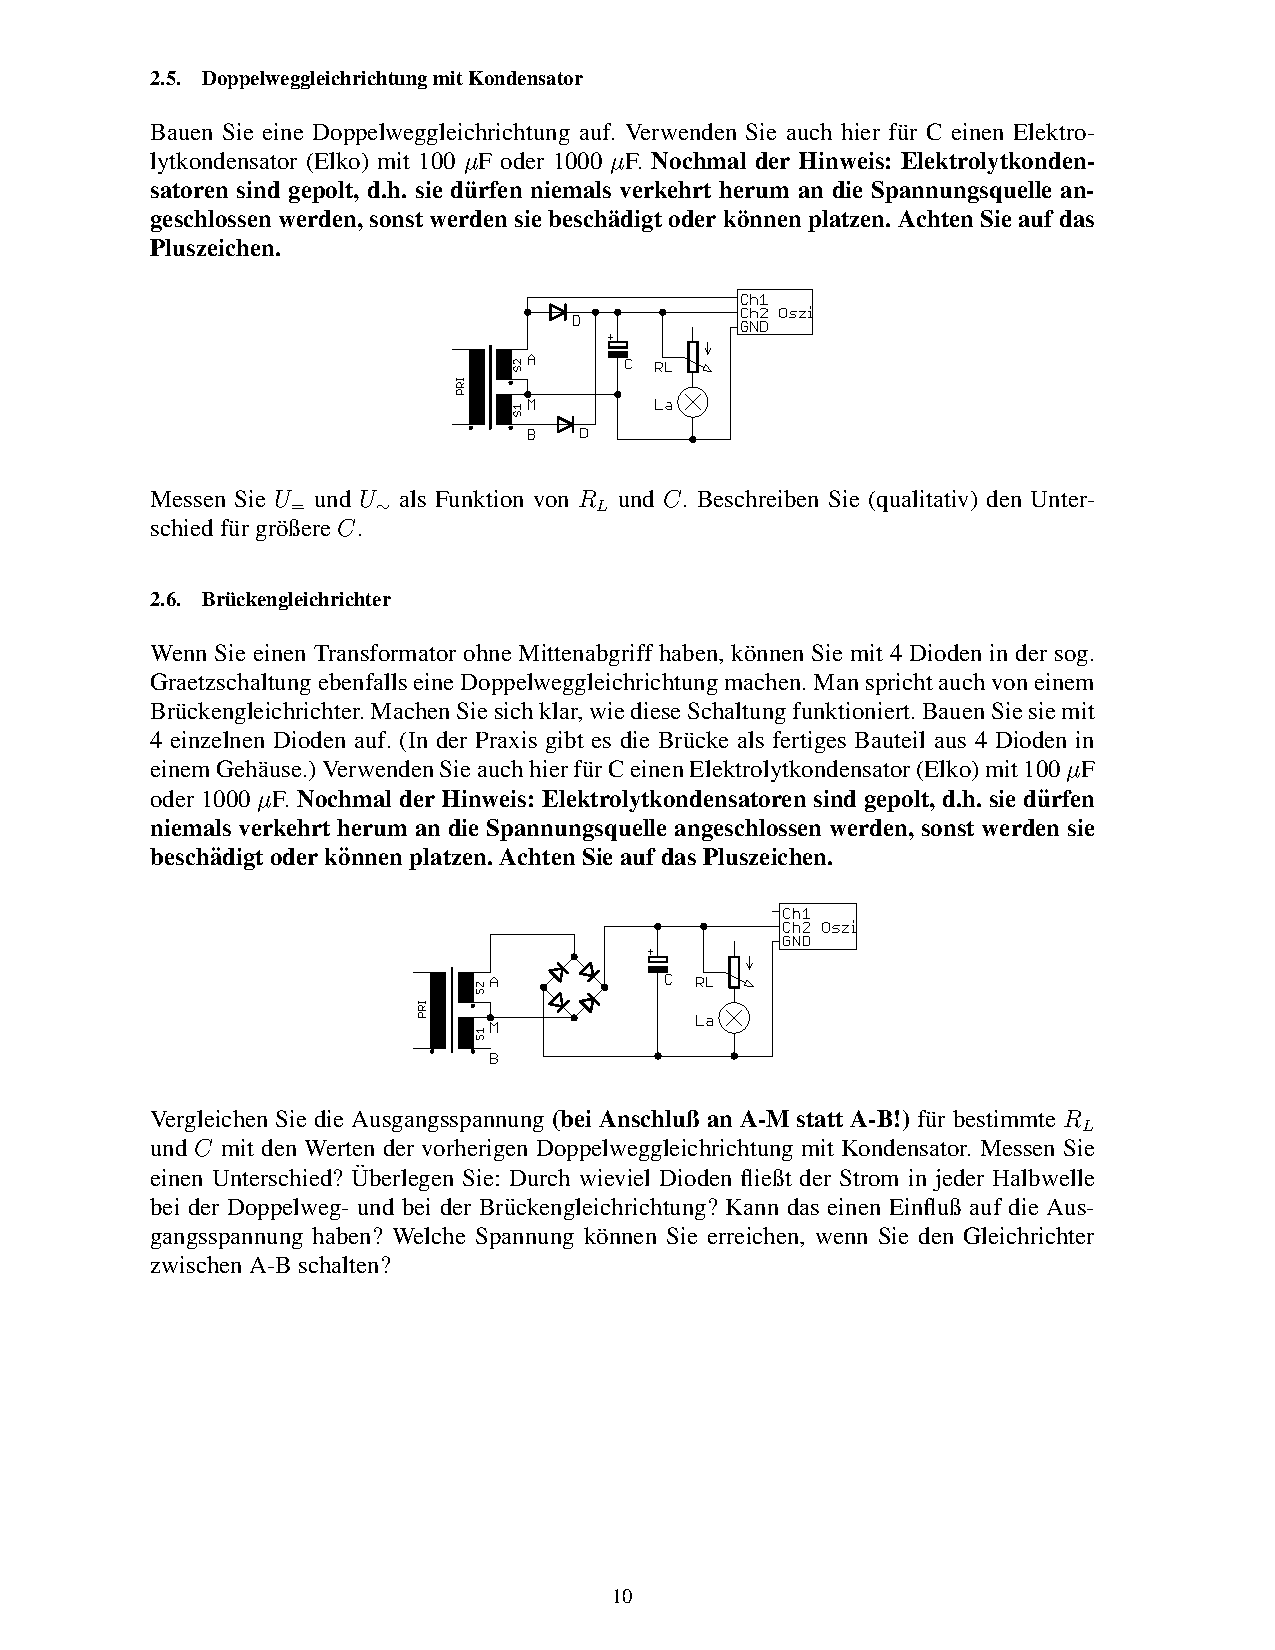
\includegraphics[trim = 10mm 100mm 10mm 150mm, clip, scale = 1]{ep2_14[Page10].pdf}
  	\caption[Schaltskizze für einen Brückengleichrichter]{Schaltskizze für einen Brückengleichrichter\footnotemark}
  \label{fig:2_7}
\end{figure}
\footnotetext{Abbildung entnommen von http://www.atlas.uni-wuppertal.de/$\sim$kind/ep2\_14.pdf Seite 10 am 28.10.2014}

\subsubsection{Versuchsdurchführung}
%erklären, !was! wir machen, !warum! wir das machen und mit welchem ziel
%(wichtig) präzize erklären, wie bei dem versuch vorgegangen und was gemacht wurde
\subsubsection{Messergebnisse}
%die messwerte in !übersichtlichen! tabellen angegeben
%zu viele kleine tabellen in große tabellen überführen!
%zu große tabellen mit dem [scale]-befehl scalieren oder (falls zu lang) in zwei kleinere tabellen aufteilen
%(wichtig) vor !jeder! tabelle sagen, was gemessen wurde und wie die fehler gewählt wurden und ausreichend !erklären!, !warum! wir unsere fehler grade so gewählt haben
\subsubsection{Auswertung}
%zuerst !alle! errechneten werte entweder in ganzen sätzen aufzählen, oder in tabellen (übersichtlicher) dargestellen, sowie auf die verwendeten formeln verweisen (die referenzierung der formel kann in der überschrift stehen)
%kurz erwähnen (vor der tabelle), warum wir das ganze ausrechnen bzw. was wir dort ausrechnen
%danach histogramme und plots erstellen, wobei wenn möglich funktionen durch die plots gelegt werden (zur not können auch splines benutzt werden, was aber angegeben werden muss)
%bei fits immer die funktion und das reduzierte chiquadrat mit angegeben, wobei auf verständlichkeit beim entziffern der zehnerpotenzen geachtet werden muss z.b. f(x)=(wert+-fehler)\cdot10^{irgendeine zahl}\cdot x + (wert+-fehler)\cdot10^{irgendeine zahl}
%bei jedem fit erklären, nach welchem zusammenhang gefittet wurde und warum!
%bei plots darauf achten, dass die achsenbeschriftung (auch die tics) die richtige größe haben und die legende im plot nicht die messwerte verdeckt
%kurz die aufgabenstellung abgehandeln
\subsection{Diskussion}
%(immer) die gemessenen werte und die bestimmten werte über die messfehler mit literaturwerten oder untereinander vergleichen
%in welchem fehlerintervall des messwertes liegt der literaturwert oder der vergleichswert?
%wie ist der relative anteil des fehlers am messwert und damit die qualität unserer messung?
%in einem satz erklären, wie gut unser fehler und damit unsere messung ist
%kurz erläutern, wie systematische fehler unsere messung beeinflusst haben könnten
%(wichtig) zum schluss ansprechen, in wie weit die ergebnisse mit der theoretischen vorhersage übereinstimmen
%--------------------------------------------------------------------------------------------
%falls tabellen mit den messwerten zu lang werden, kann die section mit den messwerten auch hinter der diskussion angefügt bzw. eine section mit dem anhang eingefügt werden.
\section{Spannungsstabilisierung}
%kurz das ziel dieses versuchsteiles ansprechen, damit keine zwei überschriften direkt übereinander stehen!
%bei schwierigeren versuchen kann auch der theoretische hintergrund erläutert werden. (mit formeln, herleitungen und erklärungen)
\subsection{Verwendete Formeln}
%eine legende kann angefertigt werden, die selbstverständlichen buchstaben müssen nicht extra erklärt werden
%mit knappen erklärungen die !verwendeten! formeln, sowie die zugehörige fehlerrechnung einfügen.
\subsection{Verwendete Materialien}
%(immer) eine skizze oder ein foto einfügen, die geräte/materialien !nummerieren! und z.b. eine legende dazu schreiben oder besser noch das ganze in einem Fließtext gut umschreiben
%falls am anfang des versuches nicht klar ist, was alles verwendet wird, wenn möglich erst am ende ein großes foto von den verwendeten materialien machen!
\subsection{Spannugsstabilisierung mit Zenerdiode (Transformatorbetrieb)}
\subsubsection{Versuchsaufbau}
%skizze zum versuchsaufbau (oder foto) einfügen,   es muss erklärt werden wie das ganze funktioniert und welche speziellen einstellungen verwendet wurden (z.b. welche knöpfe an den geräten für die messung verdreht wurden)

\begin{figure}[H] 
  \centering
    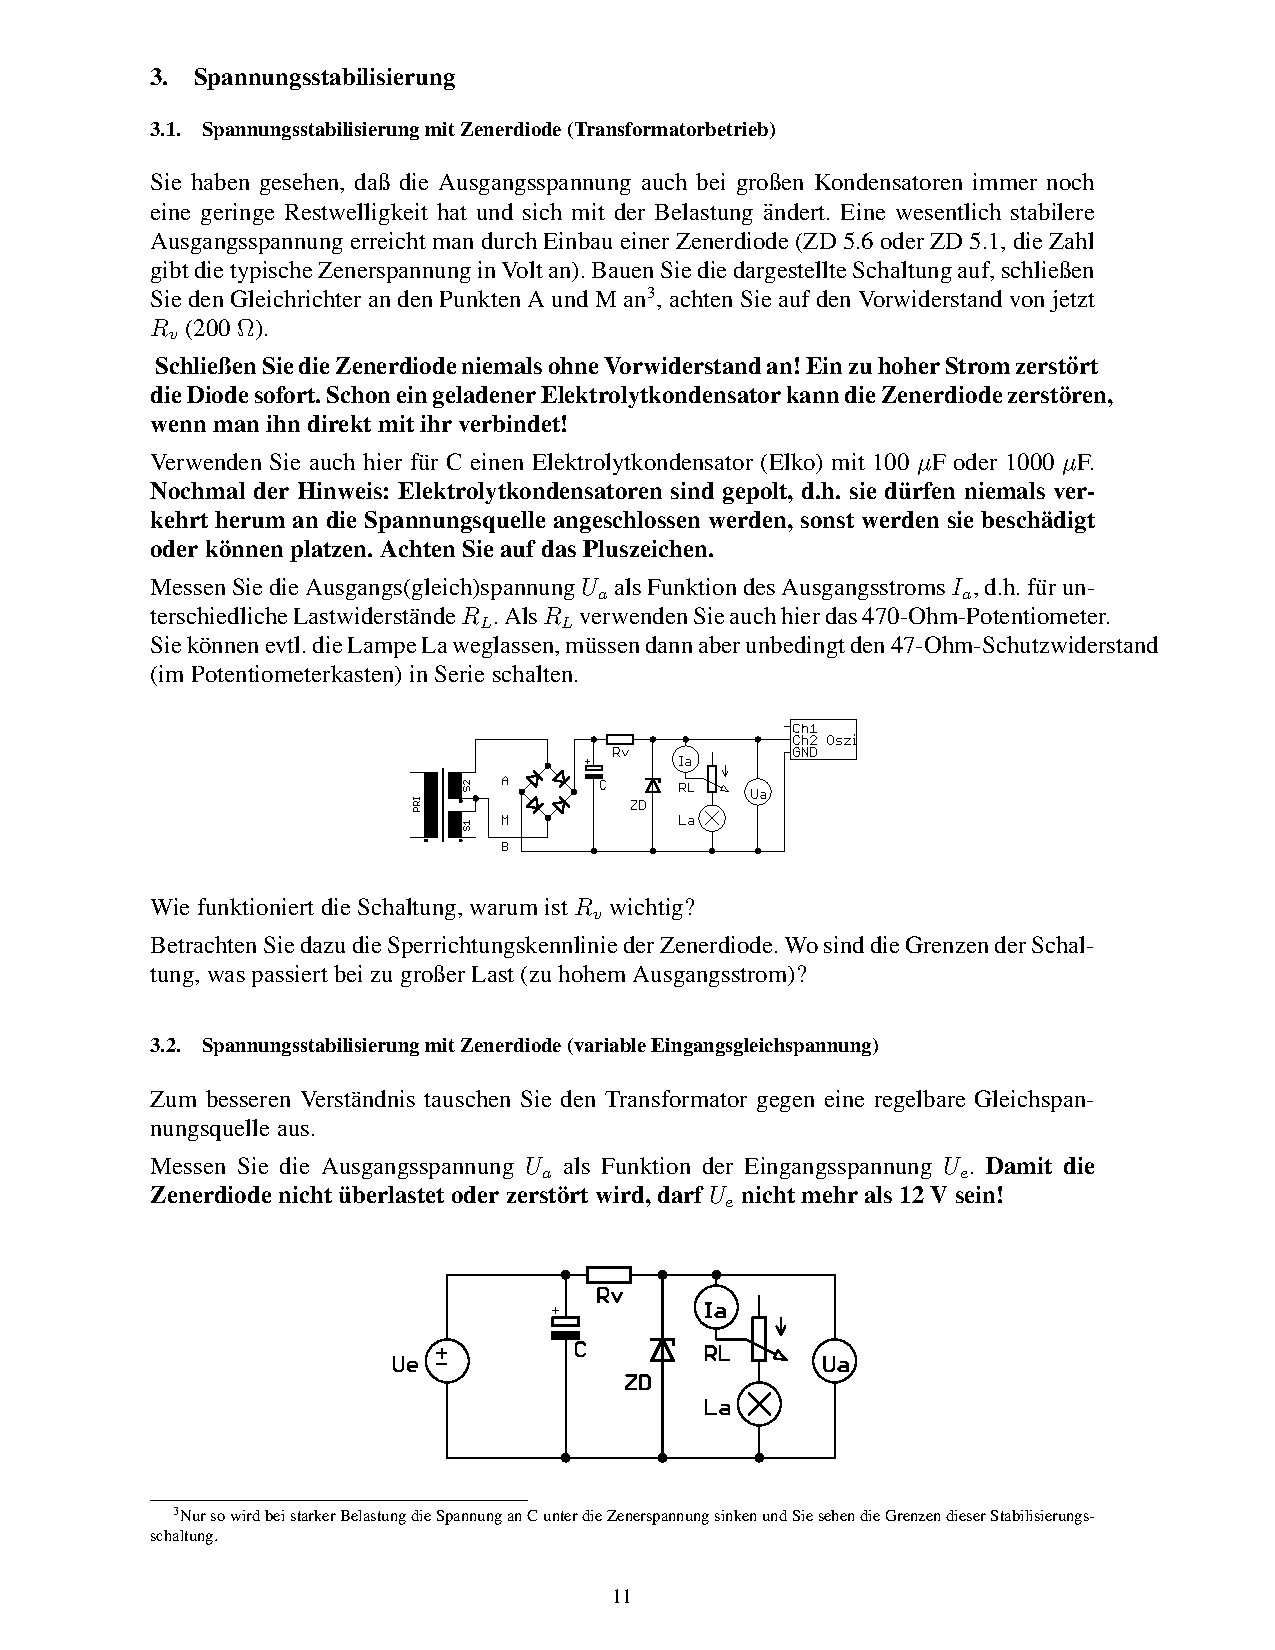
\includegraphics[trim = 10mm 130mm 10mm 120mm, clip, scale = 1]{ep2_14[Page11].pdf}
  	\caption[Schaltskizze für Schaltung zur Spannugsstabilisierung mit Zenerdiode]{Schaltskizze für Schaltung zur Spannugsstabilisierung mit Zenerdiode\footnotemark}
  \label{fig:2_8}
\end{figure}
\footnotetext{Abbildung entnommen von http://www.atlas.uni-wuppertal.de/$\sim$kind/ep2\_14.pdf Seite 10 am 28.10.2014}

\subsubsection{Versuchsdurchführung}
%erklären, !was! wir machen, !warum! wir das machen und mit welchem ziel
%(wichtig) präzize erklären, wie bei dem versuch vorgegangen und was gemacht wurde
\subsubsection{Messergebnisse}
%die messwerte in !übersichtlichen! tabellen angegeben
%zu viele kleine tabellen in große tabellen überführen!
%zu große tabellen mit dem [scale]-befehl scalieren oder (falls zu lang) in zwei kleinere tabellen aufteilen
%(wichtig) vor !jeder! tabelle sagen, was gemessen wurde und wie die fehler gewählt wurden und ausreichend !erklären!, !warum! wir unsere fehler grade so gewählt haben
\subsubsection{Auswertung}
%zuerst !alle! errechneten werte entweder in ganzen sätzen aufzählen, oder in tabellen (übersichtlicher) dargestellen, sowie auf die verwendeten formeln verweisen (die referenzierung der formel kann in der überschrift stehen)
%kurz erwähnen (vor der tabelle), warum wir das ganze ausrechnen bzw. was wir dort ausrechnen
%danach histogramme und plots erstellen, wobei wenn möglich funktionen durch die plots gelegt werden (zur not können auch splines benutzt werden, was aber angegeben werden muss)
%bei fits immer die funktion und das reduzierte chiquadrat mit angegeben, wobei auf verständlichkeit beim entziffern der zehnerpotenzen geachtet werden muss z.b. f(x)=(wert+-fehler)\cdot10^{irgendeine zahl}\cdot x + (wert+-fehler)\cdot10^{irgendeine zahl}
%bei jedem fit erklären, nach welchem zusammenhang gefittet wurde und warum!
%bei plots darauf achten, dass die achsenbeschriftung (auch die tics) die richtige größe haben und die legende im plot nicht die messwerte verdeckt
%kurz die aufgabenstellung abgehandeln
\subsection{Spannungstabilisierung mit Zenerdiode (variable Eingangsspannung)}
\subsubsection{Versuchsaufbau}
%skizze zum versuchsaufbau (oder foto) einfügen,   es muss erklärt werden wie das ganze funktioniert und welche speziellen einstellungen verwendet wurden (z.b. welche knöpfe an den geräten für die messung verdreht wurden)

\begin{figure}[H] 
  \centering
    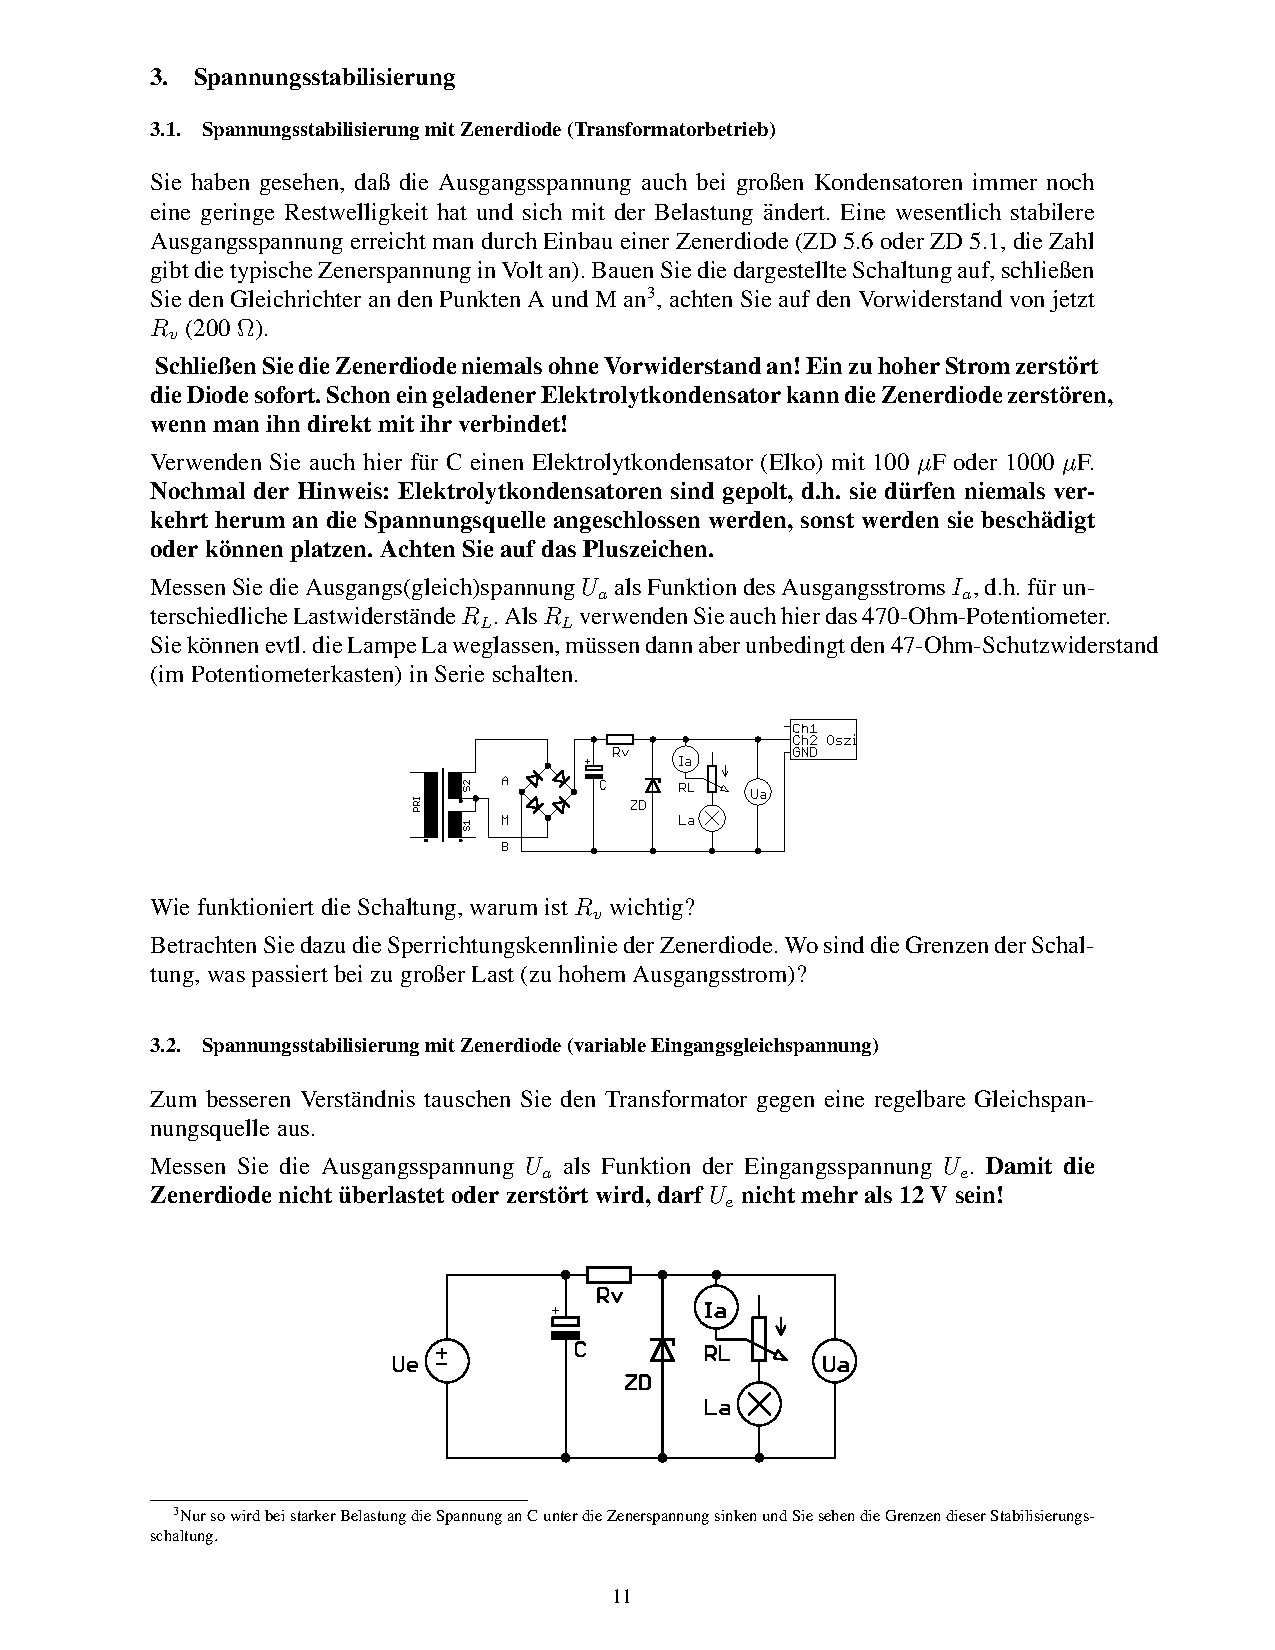
\includegraphics[trim = 10mm 30mm 10mm 213mm, clip, scale = 1]{ep2_14[Page11].pdf}
  	\caption[Schaltskizze für Schaltung zur Spannugsstabilisierung mit Zenerdiode, bei variabler Eingangsspannung]{Schaltskizze für Schaltung zur Spannugsstabilisierung mit Zenerdiode, bei variabler Eingangsspannung\footnotemark}
  \label{fig:2_8}
\end{figure}
\footnotetext{Abbildung entnommen von http://www.atlas.uni-wuppertal.de/$\sim$kind/ep2\_14.pdf Seite 10 am 28.10.2014}


\subsubsection{Versuchsdurchführung}
%erklären, !was! wir machen, !warum! wir das machen und mit welchem ziel
%(wichtig) präzize erklären, wie bei dem versuch vorgegangen und was gemacht wurde

\subsubsection{Messergebnisse}
%die messwerte in !übersichtlichen! tabellen angegeben
%zu viele kleine tabellen in große tabellen überführen!
%zu große tabellen mit dem [scale]-befehl scalieren oder (falls zu lang) in zwei kleinere tabellen aufteilen
%(wichtig) vor !jeder! tabelle sagen, was gemessen wurde und wie die fehler gewählt wurden und ausreichend !erklären!, !warum! wir unsere fehler grade so gewählt haben
\subsubsection{Auswertung}
%zuerst !alle! errechneten werte entweder in ganzen sätzen aufzählen, oder in tabellen (übersichtlicher) dargestellen, sowie auf die verwendeten formeln verweisen (die referenzierung der formel kann in der überschrift stehen)
%kurz erwähnen (vor der tabelle), warum wir das ganze ausrechnen bzw. was wir dort ausrechnen
%danach histogramme und plots erstellen, wobei wenn möglich funktionen durch die plots gelegt werden (zur not können auch splines benutzt werden, was aber angegeben werden muss)
%bei fits immer die funktion und das reduzierte chiquadrat mit angegeben, wobei auf verständlichkeit beim entziffern der zehnerpotenzen geachtet werden muss z.b. f(x)=(wert+-fehler)\cdot10^{irgendeine zahl}\cdot x + (wert+-fehler)\cdot10^{irgendeine zahl}
%bei jedem fit erklären, nach welchem zusammenhang gefittet wurde und warum!
%bei plots darauf achten, dass die achsenbeschriftung (auch die tics) die richtige größe haben und die legende im plot nicht die messwerte verdeckt
%kurz die aufgabenstellung abgehandeln
\subsection{Erhöhung des Ausgangsstroms mit Transistor}
\subsubsection{Versuchsaufbau}
%skizze zum versuchsaufbau (oder foto) einfügen,   es muss erklärt werden wie das ganze funktioniert und welche speziellen einstellungen verwendet wurden (z.b. welche knöpfe an den geräten für die messung verdreht wurden)

\begin{figure}[H] 
  \centering
    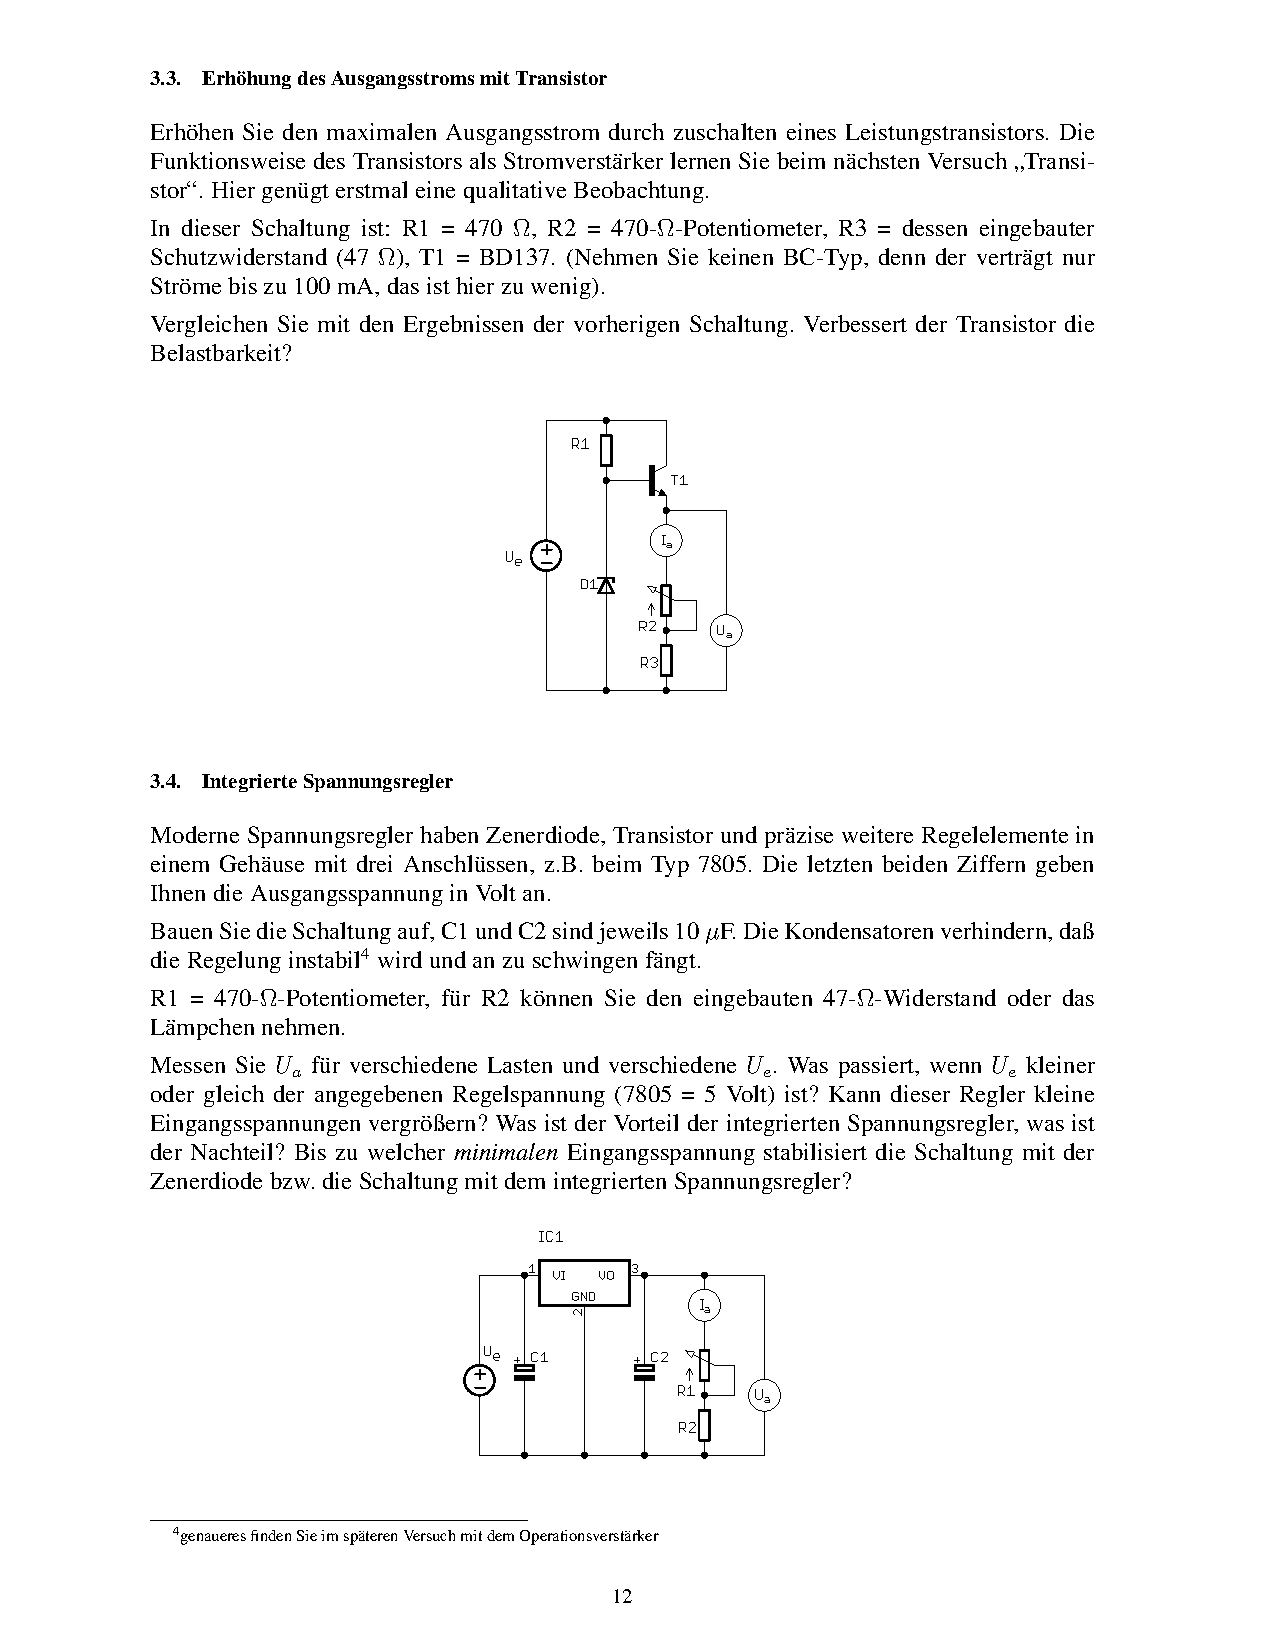
\includegraphics[trim = 10mm 160mm 10mm 70mm, clip, scale = 1]{ep2_14[Page12].pdf}
  	\caption[Schaltskizze für Schaltung zur Spannugsstabilisierung mit Zenerdiode, bei variabler Eingangsspannung]{Schaltskizze für Schaltung zur Spannugsstabilisierung mit Zenerdiode, bei variabler Eingangsspannung\footnotemark}
  \label{fig:2_8}
\end{figure}
\footnotetext{Abbildung entnommen von http://www.atlas.uni-wuppertal.de/$\sim$kind/ep2\_14.pdf Seite 10 am 28.10.2014}

\subsubsection{Versuchsdurchführung}
%erklären, !was! wir machen, !warum! wir das machen und mit welchem ziel
%(wichtig) präzize erklären, wie bei dem versuch vorgegangen und was gemacht wurde

\subsubsection{Messergebnisse}
%die messwerte in !übersichtlichen! tabellen angegeben
%zu viele kleine tabellen in große tabellen überführen!
%zu große tabellen mit dem [scale]-befehl scalieren oder (falls zu lang) in zwei kleinere tabellen aufteilen
%(wichtig) vor !jeder! tabelle sagen, was gemessen wurde und wie die fehler gewählt wurden und ausreichend !erklären!, !warum! wir unsere fehler grade so gewählt haben
\subsubsection{Auswertung}
%zuerst !alle! errechneten werte entweder in ganzen sätzen aufzählen, oder in tabellen (übersichtlicher) dargestellen, sowie auf die verwendeten formeln verweisen (die referenzierung der formel kann in der überschrift stehen)
%kurz erwähnen (vor der tabelle), warum wir das ganze ausrechnen bzw. was wir dort ausrechnen
%danach histogramme und plots erstellen, wobei wenn möglich funktionen durch die plots gelegt werden (zur not können auch splines benutzt werden, was aber angegeben werden muss)
%bei fits immer die funktion und das reduzierte chiquadrat mit angegeben, wobei auf verständlichkeit beim entziffern der zehnerpotenzen geachtet werden muss z.b. f(x)=(wert+-fehler)\cdot10^{irgendeine zahl}\cdot x + (wert+-fehler)\cdot10^{irgendeine zahl}
%bei jedem fit erklären, nach welchem zusammenhang gefittet wurde und warum!
%bei plots darauf achten, dass die achsenbeschriftung (auch die tics) die richtige größe haben und die legende im plot nicht die messwerte verdeckt
%kurz die aufgabenstellung abgehandeln
\subsection{Integrierte Spannungsregler}
\subsubsection{Versuchsaufbau}
%skizze zum versuchsaufbau (oder foto) einfügen,   es muss erklärt werden wie das ganze funktioniert und welche speziellen einstellungen verwendet wurden (z.b. welche knöpfe an den geräten für die messung verdreht wurden)

\begin{figure}[H] 
  \centering
    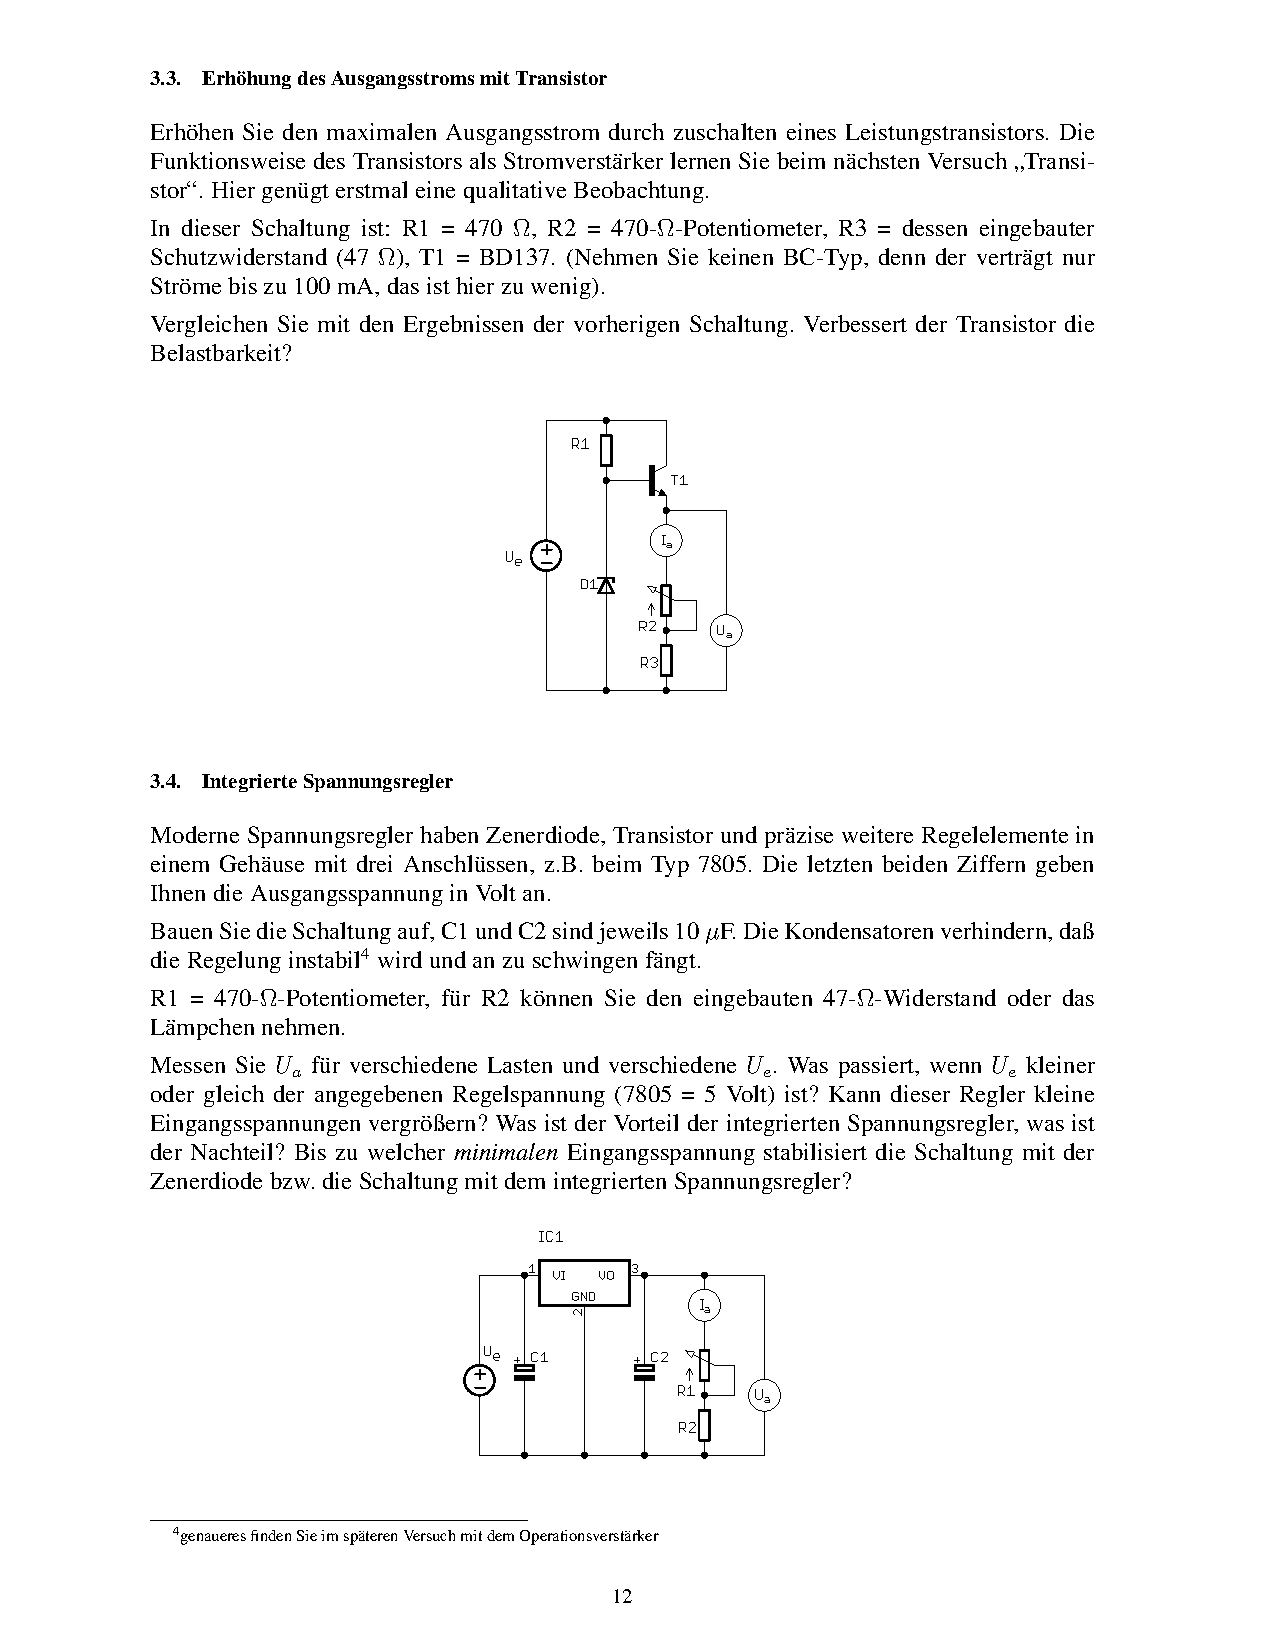
\includegraphics[trim = 10mm 30mm 10mm 205mm, clip, scale = 1]{ep2_14[Page12].pdf}
  	\caption[Schaltskizze für Schaltung zur Spannugsstabilisierung mit Zenerdiode, bei variabler Eingangsspannung]{Schaltskizze für Schaltung zur Spannugsstabilisierung mit Zenerdiode, bei variabler Eingangsspannung\footnotemark}
  \label{fig:2_8}
\end{figure}
\footnotetext{Abbildung entnommen von http://www.atlas.uni-wuppertal.de/$\sim$kind/ep2\_14.pdf Seite 10 am 28.10.2014}

\subsubsection{Versuchsdurchführung}
%erklären, !was! wir machen, !warum! wir das machen und mit welchem ziel
%(wichtig) präzize erklären, wie bei dem versuch vorgegangen und was gemacht wurde

\subsubsection{Messergebnisse}
%die messwerte in !übersichtlichen! tabellen angegeben
%zu viele kleine tabellen in große tabellen überführen!
%zu große tabellen mit dem [scale]-befehl scalieren oder (falls zu lang) in zwei kleinere tabellen aufteilen
%(wichtig) vor !jeder! tabelle sagen, was gemessen wurde und wie die fehler gewählt wurden und ausreichend !erklären!, !warum! wir unsere fehler grade so gewählt haben
\subsubsection{Auswertung}
%zuerst !alle! errechneten werte entweder in ganzen sätzen aufzählen, oder in tabellen (übersichtlicher) dargestellen, sowie auf die verwendeten formeln verweisen (die referenzierung der formel kann in der überschrift stehen)
%kurz erwähnen (vor der tabelle), warum wir das ganze ausrechnen bzw. was wir dort ausrechnen
%danach histogramme und plots erstellen, wobei wenn möglich funktionen durch die plots gelegt werden (zur not können auch splines benutzt werden, was aber angegeben werden muss)
%bei fits immer die funktion und das reduzierte chiquadrat mit angegeben, wobei auf verständlichkeit beim entziffern der zehnerpotenzen geachtet werden muss z.b. f(x)=(wert+-fehler)\cdot10^{irgendeine zahl}\cdot x + (wert+-fehler)\cdot10^{irgendeine zahl}
%bei jedem fit erklären, nach welchem zusammenhang gefittet wurde und warum!
%bei plots darauf achten, dass die achsenbeschriftung (auch die tics) die richtige größe haben und die legende im plot nicht die messwerte verdeckt
%kurz die aufgabenstellung abgehandeln
\subsection{Diskussion}
%(immer) die gemessenen werte und die bestimmten werte über die messfehler mit literaturwerten oder untereinander vergleichen
%in welchem fehlerintervall des messwertes liegt der literaturwert oder der vergleichswert?
%wie ist der relative anteil des fehlers am messwert und damit die qualität unserer messung?
%in einem satz erklären, wie gut unser fehler und damit unsere messung ist
%kurz erläutern, wie systematische fehler unsere messung beeinflusst haben könnten
%(wichtig) zum schluss ansprechen, in wie weit die ergebnisse mit der theoretischen vorhersage übereinstimmen
%--------------------------------------------------------------------------------------------
%falls tabellen mit den messwerten zu lang werden, kann die section mit den messwerten auch hinter der diskussion angefügt bzw. eine section mit dem anhang eingefügt werden.
\section{Fazit}
%im fazit nochmal alles zusammenfassen und den verlauf der messung abschätzen
%gravierende sytematische probleme bei den messungen nochmal betonen und die wertigkeit unserer ergebnisse einordnen
\end{document}

